
\chapter{Friction}\label{chap:friction} 
Since we aim for controlling frictional properties, we will review the relevant theoretical understanding of friction in this chapter. We limit ourselves to the tribological subcategory, wear-less dry friction, meaning that we consider friction in the absence of lubricant and wear between the contacting surfaces. We will direct the review towards our system of interest which will serve as a basis for a formal definition of our research questions at the end of this chapter.



% https://www.sciencedirect.com/science/article/abs/pii/S0301679X18300756 <----- READ
\section{Friction across scales}
Tribological systems span a wide range of time and length scales, from
geological stratum layers involved in earthquakes~\cite{kim_nano-scale_2009} to
atomistic processes, such as the gliding motion of nanoclusters or nanomotors
\cite{Manini_2016}. This vast difference in scale leads to different dominant
frictional mechanisms. At the macroscale, the experimental systems are typically subjected to relatively high loads and sliding speeds, resulting in significant contact stress and wear. This makes for a macroscale friction that is often reduced into a few variables such as load, material type, sliding speed and surface roughness. On the other hand, the micro-/nanoscale regime is usually studied in the opposite domain operating under a relatively small load and sliding speed with negligible wear~\cite{kim_nano-scale_2009}~\cite[p. 5]{bhushan_2013}. This reveals a change in the dominant mechanism at play with an emphasis on the importance of surface properties. The works of Bhushan and Kulkarni~\cite{BHUSHAN199649} showed that the friction coefficient decreased with scale even though the materials used were unchanged. This reveals an intrinsic relationship between friction and scale as the contact condition is altered. The phenomenological descriptions of macroscale friction cannot yet be derived
from the fundamental atomic principles, and bridging the gap between different
length scales in tribological systems remains an open challenge
\cite{Manini_2016}. Hence, the following sections will be organized into
macroscale (\cref{sec:macroscale}), microscale (\cref{sec:microscale}) and
nanoscale (\cref{sec:nanoscale}) representing the theoretical understanding
governing each scale regime. Realizing that the field of friction across all
scales is a vastly broad topic, we will only introduce the most essential findings for each scale while keeping a main focus on features associated with our system on at the nanoscale.


% The differences between the conventional or macro tribology and
% micro/nanotribology are contrasted in Figure 1.3.1. In macro tribology, tests
% are conducted on components with relatively large mass under heavily loaded
% conditions. In these tests, wear is inevitable and the bulk properties of
% mating components dominate the tribological performance. In
% micro/nanotribology, measurements are made on components, at least one of the
% mating components, with relatively small mass under lightly loaded conditions.
% In this situation, negligible wear occurs and the surface properties dominate
% the tribological performance.~\cite{bhushan_2013}[p. 5]



% We were astonished to discover that molecules that could flex or slide even
% just a little in response to the oscillatory motion of the microbalance were
% linked to low friction levels at the macro-scale. Put another way,
% exceptionally low friction at the atomic scale was not a prerequisite for the
% substantial reduction in macroscopic friction.
% (\url{https://physicsworld.com/a/friction-at-the-nano-scale/})



% It is generally accepted that friction is caused by more than one mechanism in
% a given sliding system. Generally, a frictional force arises due to two
% fundamentally different causes, namely one that is mechanical in nature and
% the other being chemical in its origin. In the case of the mechanical cause of
% friction, plowing of the surface by hard particles or asperities is mainly
% responsible for generating the frictional force.2,4,5-7 As for the chemical
% mechanism of friction, adhesion between surfaces of the two solids in contact
% is the cause of friction.2,4,5,8 Another point to note is that tribological 
% phenomenon are heavily dependent on system parameters of the operating machine
% such as speed, temperature, load, and environment. As such, the dominating.
%~\cite{kim_nano-scale_2009}.




\section{Macroscale}\label{sec:macroscale}
Our working definition of the \textit{macroscale} is everything on the scale of millimeters and above~\cite{HUNG2015215}. This represents the scale of visible objects and includes objects from everyday interactions to big geological systems. 

% Most importantly, we want to make a distinction to the microscale, where the prefix indicates the size of micrometers $m^{-6}$. Hence, we consider everything larger than \textit{micro} to belong to the macroscale\footnote{The width of a human hair is often used as a reference for the limit of human perception. Since the width of a human hair is on the length scale $10^{-5}$ to \SI{e-4}{m} we find this limit aligns rather well with the defined transition from macro- to microscale.}.



\subsection{Amontons’ law}
% Based on~\cite{gnecco_meyer_2015}
% and~\cite{gao_frictional_2004}
In order to start and keep a solid block moving against a solid surface we must
overcome certain frictional forces $F_{\text{fric}}$~\cite{gnecco_meyer_2015}.
The static friction force $F_s$ corresponds to the minimum tangential force
required to initiate the sliding while the kinetic friction force $F_k$
corresponds to the tangential force needed to sustain such a sliding at a steady
speed. The work of Leonardo da Vinci (1452–-1519), Guillaume Amontons (1663--705)
and Charles de Coulomb (1736--1806) all contributed to the empirical law,
commonly known as \textit{Amontons’ law}, which serves as a common base for macroscale
friction. Amontons’ law states that the frictional forces are entirely
independent of contact area and sliding velocity. Instead, it relies only on
the normal force $F_N$, acting perpendicular to the surface, and the material-specific friction coefficient $\mu$ as
\begin{align}
  F_{\text{fric}} = \mu F_N.
  \label{eq:amonton}
\end{align}
Notice that the term \textit{normal force} is often used interchangeably with \textit{load} and \textit{normal load} although the load and normal load refer to the applied force that pushes the object into the surface, whereas the normal force is the reaction force acting from the surface on the object. In equilibrium, these forces are equal in magnitude and opposite in direction, and for the scope of our thesis, we will not make a distinction between these terms as well. On the same note, we point out that the frictional force is different from a conventional force which in the Newtonian definition acts on a body from the outside and makes it accelerate~\cite{gao_frictional_2004}. Rather than being an independent external force the friction force is an internal \textit{reaction} force opposing the externally applied ``sliding'' force. 

The friction coefficient $\mu$ is typically different for the cases of static
($\mu_s$) and kinetic ($\mu_k$) friction, usually both with values lower than
one and $\mu_s \ge \mu_k$ in all cases~\cite[p. 6]{gnecco_meyer_2015}. The friction coefficient is taken to be a constant defined by either~\cite{gao_frictional_2004} \\
\vspace{0.1cm}
\begin{subequations}
\noindent\begin{minipage}{.2\linewidth}
  \hfill
\end{minipage}
\begin{minipage}[b]{0.2\linewidth}
  \begin{align}
    \mu_1 = \frac{F_{\text{fric}}}{F_N},
    \label{eq:mu_def1}
  \end{align}
\end{minipage}
\begin{minipage}[b]{0.2\linewidth}
  \begin{align*}
    \text{or}
  \end{align*}
\end{minipage}
\begin{minipage}[b]{0.2\linewidth}
  \begin{align}
    \mu_2 = \frac{dF_{\text{fric}}}{dF_N}.
    \label{eq:mu_def2}
  \end{align}
\end{minipage}
\begin{minipage}{.2\linewidth}
\end{minipage}
\label{eq:mu_def}
\end{subequations}
\vspace{0.1cm}
\\
\noindent The first definition~\cref{eq:mu_def1} requires zero friction at zero
load, i.e.\ $F_{\text{fric}} = 0$ at $F_N = 0$, while the second definition~\cref{eq:mu_def2} allows for a finite friction force at zero load as the
coefficient is defined by the slope of the friction-load curve. The
consequences of these definitions are illustrated in~\cref{fig:fric_coef_example}, for selected friction-load-curves in~\cref{fig:fric_coef_example_a} and corresponding friction coefficients in~\cref{fig:fric_coef_example_b} and~\cref{fig:fric_coef_example_c}. For adhesive
contacts, the friction force will not be zero under zero load~\cite{gao_frictional_2004} (red curve: Linear
+ shift) which can be mitigated by adding an extra constant to~\cref{eq:amonton}. Using \cref{eq:mu_def1} for adhesive contacts would make the friction coefficient diverge for decreasing load as illustrated in~\cref{fig:fric_coef_example_b}. Thus, we find the second
definition~\cref{eq:mu_def2} more robust and versatile. This also allows for a better interpretation of the friction coefficient in the case where
friction depends non-linearly on load as seen with the purple curve in~\cref{fig:fric_coef_example}. 


% In reality the friction coefficient is not truly a
% material-specific constant as it is often found to vary under different
% conditions such as humidity or smooth and rough morphologies of the sliding
% surfaces~\cite{gao_frictional_2004}.


\begin{figure}[H]
  \centering
  \begin{subfigure}[t]{0.32\textwidth}
      \centering
      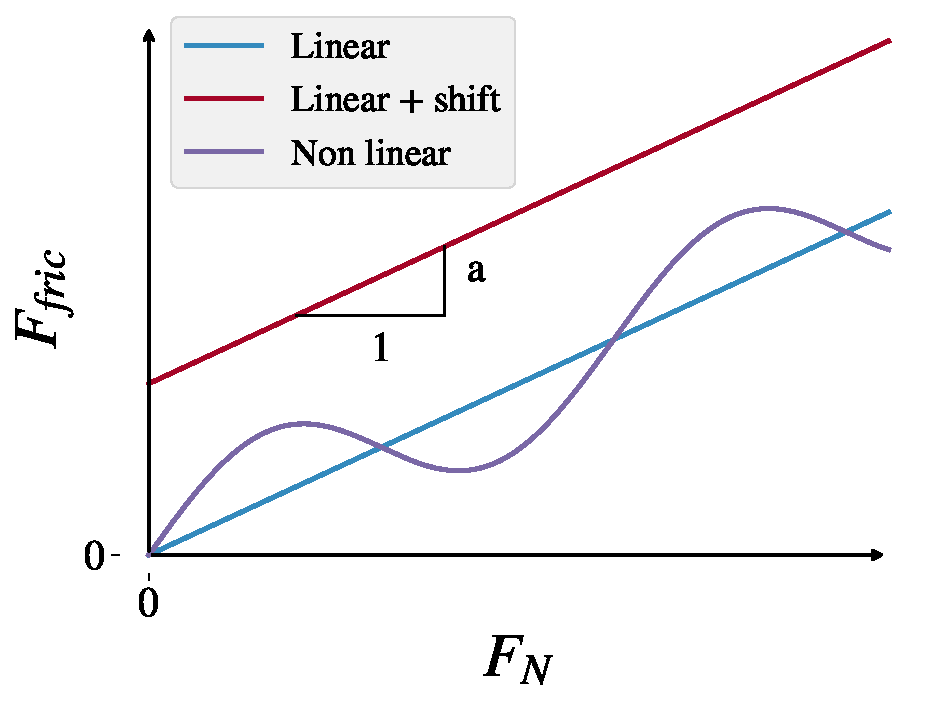
\includegraphics[width=\textwidth]{figures/theory/fric_coef_example_a.pdf}
      \caption{}
      \label{fig:fric_coef_example_a}
    \end{subfigure}
    \hfill
    \begin{subfigure}[t]{0.32\textwidth}
      \centering
      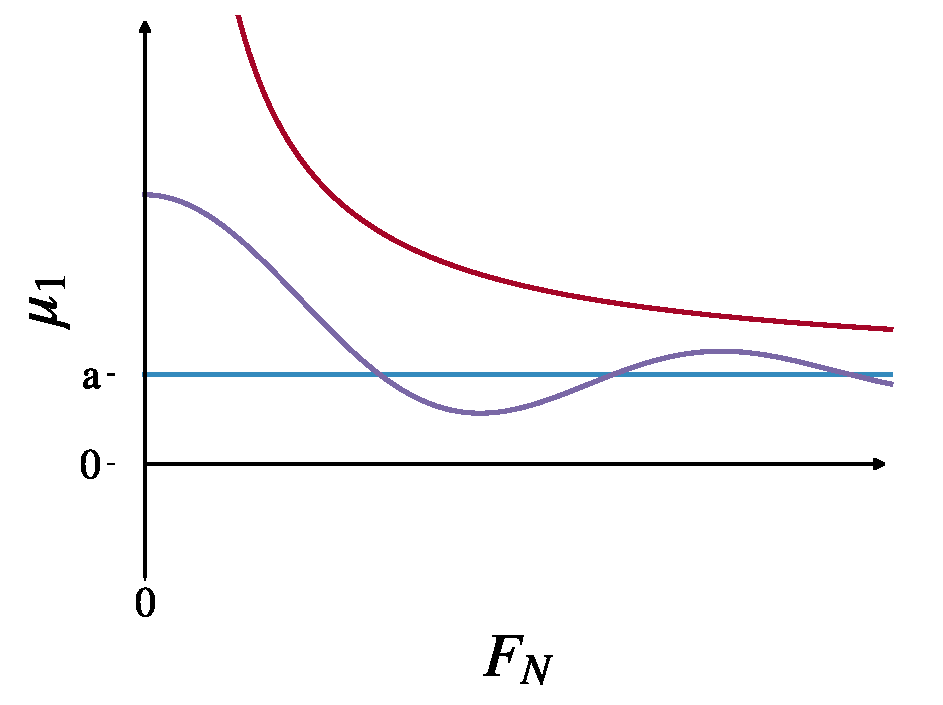
\includegraphics[width=\textwidth]{figures/theory/fric_coef_example_b.pdf}
      \caption{}
      \label{fig:fric_coef_example_b}
    \end{subfigure}
    \hfill
    \begin{subfigure}[t]{0.32\textwidth}
      \centering
      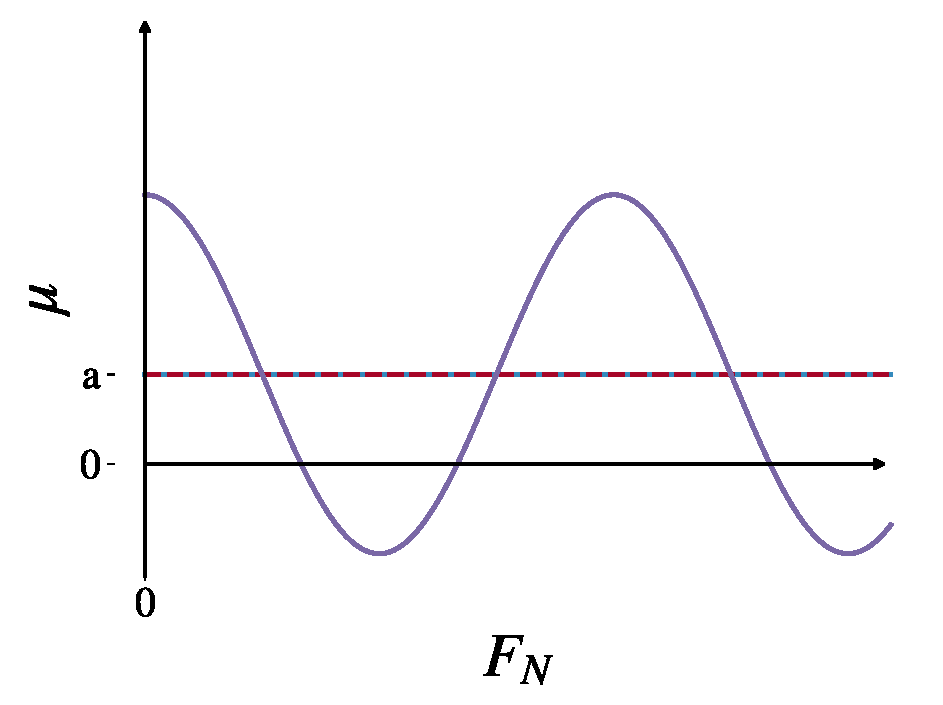
\includegraphics[width=\textwidth]{figures/theory/fric_coef_example_c.pdf}
      \caption{}
      \label{fig:fric_coef_example_c}
  \end{subfigure}
  \hfill
  \caption{Illustration of the consequences for the two definitions of the friction coefficient in~\cref{eq:mu_def}. (a) Three examples of friction-load curves consisting of a typical linear curve (blue), a linear curve with a shift representing an adhesive contact (red), and a non-linear curve (purple). The corresponding friction coefficients $\mu_1$ and $\mu_2$ are shown for the first definition \cref{eq:mu_def1} in (b) and the second definition \cref{eq:mu_def1} in (c).}
  \label{fig:fric_coef_example}
\end{figure}

% (b) The friction coefficient $\mu_1$ by definition of~\cref{eq:mu_def1}. (c) The friction coefficient $\mu_2$ by definition of~\cref{eq:mu_def2}

Amontons’ law represents the behavior relatively accurately for many surfaces in contact, involving both dry and lubricated, ductile and brittle and rough and smooth surfaces (as long as they are not adhesive) under a variety of conditions~\cite{gao_frictional_2004}. But it has its limitations. For instance, at low velocities, Amontons' model breaks down due to thermal effects, and for high velocities due to inertial effects~\cite[pp.\ 5--6]{gnecco_meyer_2015}. Additionally, static friction depends on the so-called contact history, with increasing static friction as the logarithm of time in stationary contact~\cite{dieterich_1972}.

In cases where Amontons' law breaks down, we might still use the conceptual
definition of the friction coefficient as defined by~\cref{eq:mu_def2}.
Especially, in the context of achieving negative friction coefficients (for certain load ranges), we would refer to this definition, since \cref{eq:mu_def1}
would imply a truly unphysical situation of the frictional force acting in the
same direction as the sliding motion. This would accelerate the object
indefinitely\footnote{You would most likely have a good shot at the Nobel Prize
with that paper.}.

Due to the empirical foundation of Amontons’ law, it does not provide any
physical insight into the underlying mechanisms of friction. However, as we will
later discuss in more detail, we can understand the overall phenomena of
friction through statistical mechanics by the concept of \textit{equipartition
of energy}~\cite{Manini_2016}. A system in equilibrium has its kinetic energy
uniformly distributed among all its degrees of freedom. When a macroscale object
is sliding in a given direction it is clearly not in equilibrium since one of
its degrees of freedom carries considerably more kinetic energy. Thus, the
system will tend to transfer kinetic energy to the remaining
degrees of freedom in the form of heat dissipating to the surroundings. This will make the object slow down if not continuously driven forward by an external energy source. Hence, we can understand the overall concept of friction simply
as the tendency of going toward equilibrium energy equipartitioning among many
interacting degrees of freedom~\cite{Manini_2016}. From this point of view, it is
clear that friction is an inevitable part of contact physics, but even though
friction cannot be removed altogether, we are still capable of manipulating it
in useful ways. \\
\\
The attentive reader might point out that we have already moved the discussion
into the microscopic regime as \textit{statistical mechanics} generally
aim to explain macroscale behavior by microscopic interactions. This 
highlights the necessity to consider smaller scales in order to achieve a more fundamental understanding of friction.
\\
\\
We note that more advanced models for macroscale friction exist. For instance, the earthquake-like (EQ) model, also known as the \textit{spring-and-block} model or the \textit{multi-contact} model~\cite{Manini_2016}, developed by Burridge and Knopoff~\cite{Burridge_1967}. This has been used in many studies of earthquake friction~\cite{PhysRevLett.88.096102} and similar schemes have since been used to model the failure of fiber bundles and faults~\cite{newman_failure_1991, Smalley_1985}. Also, \textit{rate and state} models have been used for such macroscale modeling modeling~\cite{SELVADURAI2023229689}. However, these extensions are beyond the scope of this thesis as we will mainly focus on the nanoscale description. 



% All the terms in Amontons’ law refer to macroscopic, i.e., space- and time-averaged or “mean-field”, values. Thus, the contact area is the “apparent” or projected geometric area rather than the “real” contact area at the molecular level. And V is the mean relative velocity of the sliding bodies even though the shearing micro junctions may be moving with large fluctuations or in a stick-slip fashion.10~\cite{gao_frictional_2004}




% This includes taking the microscopic roughness
% into account together with surface chemistry. This more complex perspective
% introduces new (...() as real contact area, contact stresses, surface adhesion
% which makes frictional properties dependent on sliding speed, temperature and
% environment in general~\cite{kim_nano-scale_2009}. 


% The conclusion is that the friction coefficient is not an intrinsic physical
% property~\cite{Szlufarska_2008}.

% The basic difficulty of friction is intrinsic, involving the dissipative
% dynamics of large systems, often across ill-characterized interfaces, and
% generally violent and nonlinear~\cite{Manini_2016}


% The severity of the task is also related to the experimental difficulty to
% probe systems with many degrees of freedom under forced spatial confinement,
% that leaves very limited access to probing the buried sliding interface.
% Thanks to remarkable developments in nanotechnology, new inroads are being
% pursued and new discoveries are being made.~\cite{Manini_2016}


\section{Microscopic scale}\label{sec:microscale}
Going from a macro- to a microscale perspective, at a length scale on the order
\SI{e-6}{m}, it was realised that most surfaces are in fact rough~\cite{mo_friction_2009}. The contact between two surfaces consists of numerous
smaller contact points, so-called \textit{asperities}, which form junctions due to contact pressure and adhesion as visualized in~\cref{fig:asperity_contact}~\cite{kim_nano-scale_2009}. In the macroscale perspective of Amonton's law, we refer to time- and space-averaged values, i.e.\ the apparent contact area and the average
sliding speed~\cite{gao_frictional_2004}. However, microscopically we find the
real contact area to be much smaller than the apparent area~\cite{kim_nano-scale_2009}, and the shearing motion of local microjunctions to happen at large fluctuations rather than as one synchronized movement throughout the surface. 

It is generally accepted that friction is caused by two mechanisms: Mechanical
friction and chemical friction~\cite{kim_nano-scale_2009}. Mechanical
friction is the ``plowing'' of the surface by hard particles or said asperities
with an energy loss attributed to deformations of the asperity. While plastic
deformations, corresponding to wear, gives rise to an obvious attribution for
the energy loss, elastic deformations are also sufficient in explaining energy
loss due to phonon excitations. The assumption of plastic deformations
has been criticized as this is theorized only to be present at the beginning of
a surface contact while it is negligible for prolonged or repeated contacts
\cite{CARBONE20082555}. That is, when machine parts slide against each other for
millions of cycles, the plastic deformation would only take place at the beginning for which the system then reaches a steady state with only elastic deformations.
The chemical friction arises from adhesion between microscopic contacting
surfaces, with an energy loss attributed to the breaking and forming of chemical bonds between the interacting surfaces. 



\subsection{Asperity theories} % Surface roughness --- Asperity theories
% Sources in general:~\cite{mo_friction_2009},~\cite{kim_nano-scale_2009} \\

Asperity theories have their foundations in the adhesion model proposed by Bowden and Tabor~\cite{bowden2001friction} which is based on the fundamental reasoning that friction is governed by the adhesion between two surfaces~\cite{Kim_2012}. Adhesion is proportional to the real contact area defined by asperity junctions, and interfacial shear strength $\vec{\tau}$ between such contacting junctions. For an asperity contact area $A_{\text{asp}}$ we get a true contact area $\sum A_{\text{asp}}$ leading to 
\begin{align*}
  F_\text{fric} = \vec{\tau} \sum A_{\text{asp}}.
\end{align*}
Note that this is still compatible with Amontons’ law in~\cref{eq:amonton} by having a linear relationship between the real contact area and the
applied load. In fact, this is exactly how the theoretical model explains the friction dependency of load. By increasing the normal load it is hypothesized that the real contact area will increase as the asperity tips are deformed (plastically or elastically) into broader contact points as visualized qualitatively in~\cref{fig:asperity_contact}.

\begin{figure}[H]
  \centering
  \begin{subfigure}[b]{0.49\textwidth}
      \centering
      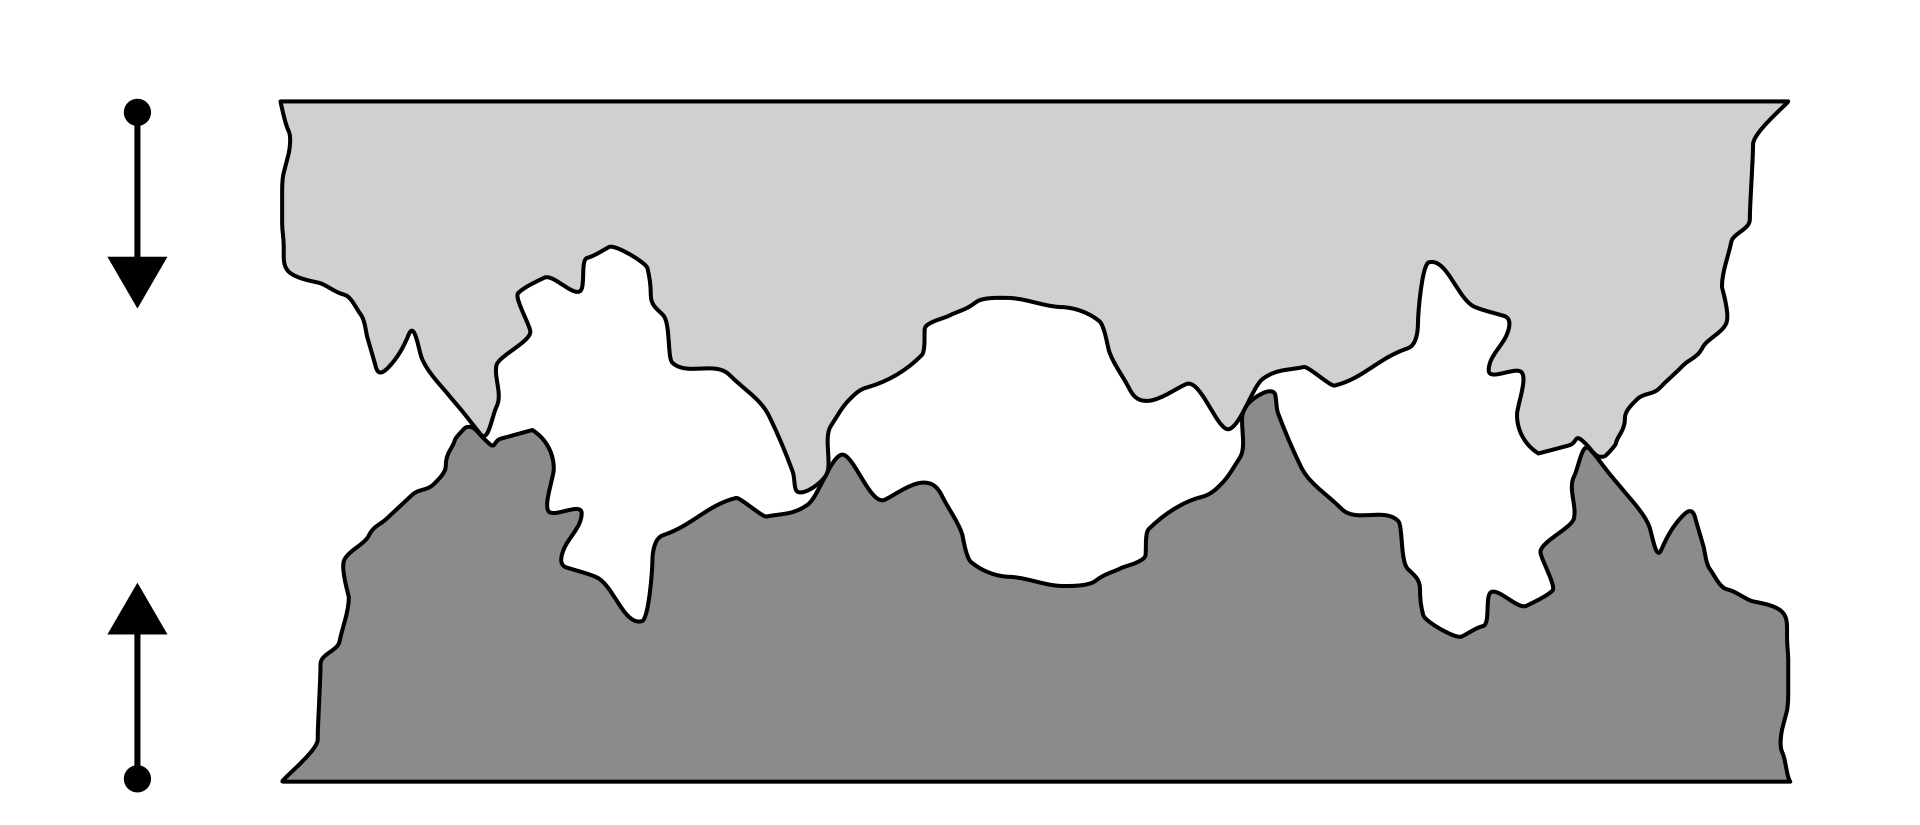
\includegraphics[width=\textwidth]{figures/theory/asperities_top.png}
      \caption{Low load.}
      \label{fig:asp_left}
  \end{subfigure}
  \hfill
  \begin{subfigure}[b]{0.49\textwidth}
      \centering
      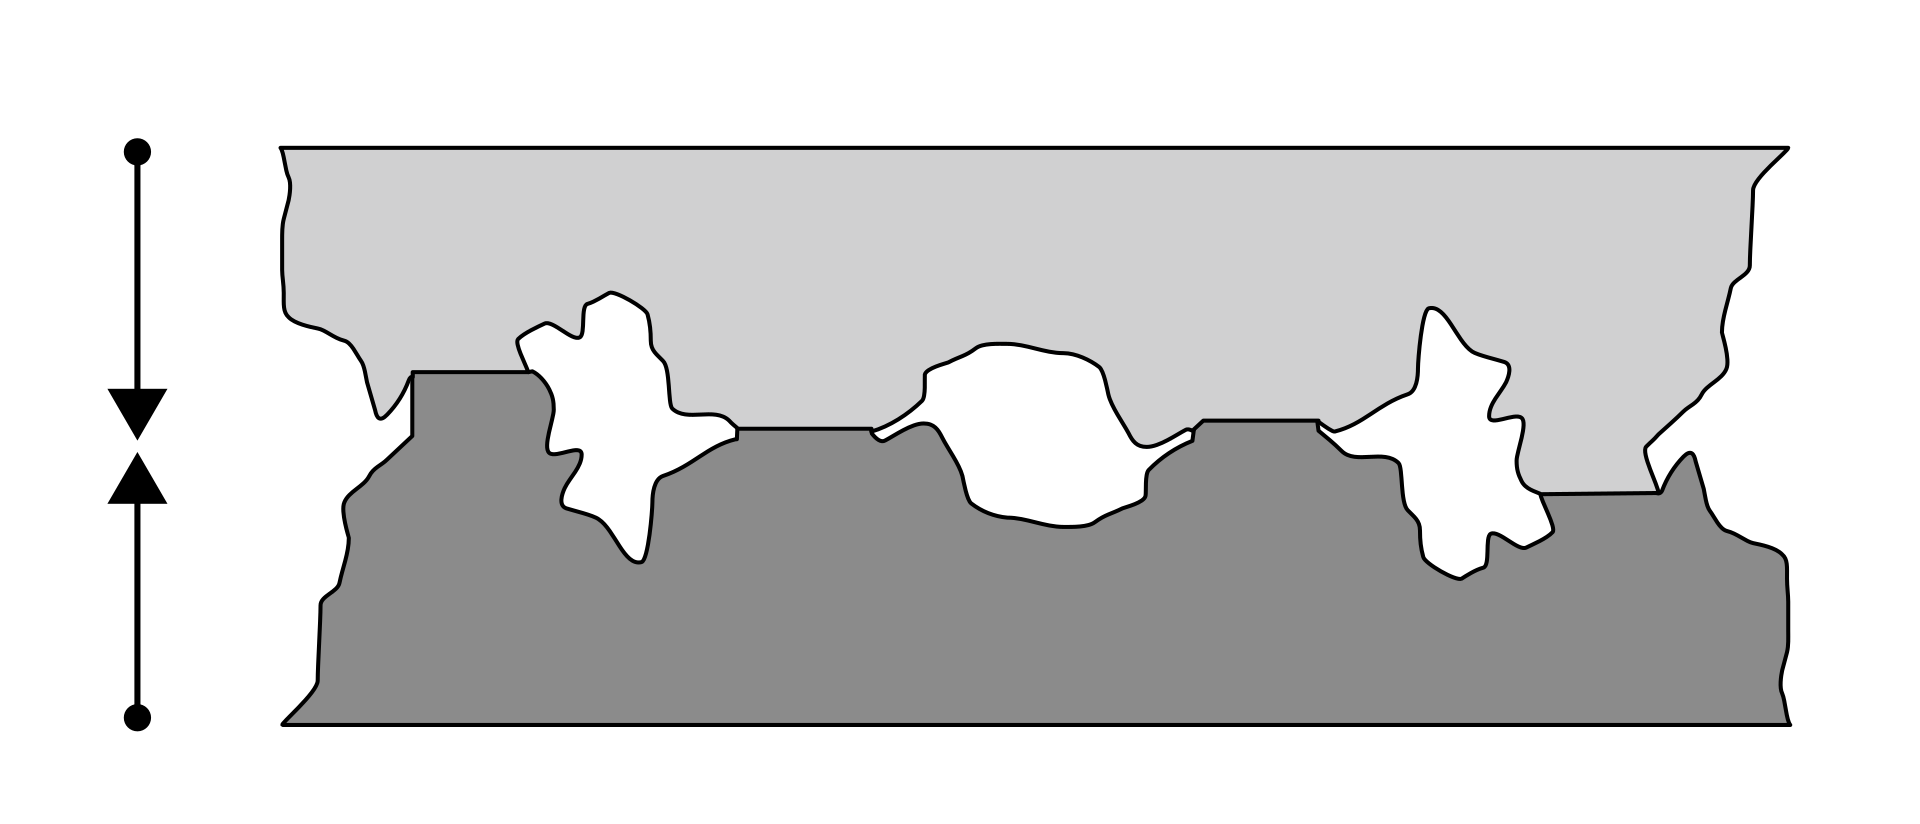
\includegraphics[width=\textwidth]{figures/theory/asperities_bottom.png}
      \caption{High load.}
      \label{fig:asp_right}
  \end{subfigure}
  \hfill
     \caption{Qualitatively illustration of the microscopic asperity deformation
     under increasing load from frame (a) to (b)~\cite{wiki:asperities}. While this figure seemingly portrays plastic deformation the concept of increased contact area with increased load applies to elastic deformation as well.}
     \label{fig:asperity_contact}
\end{figure}

Many studies have focused on single asperity contacts to reveal the relationship
between the contact area and load~\cite{Szlufarska_2008, PhysRevLett.56.930,
perry_scanning_2004}. By assuming perfectly smooth asperities, with radii of
curvature from micrometers all the way down to nanometers, continuum mechanics
can be used to predict the deformation of asperities as load is applied. A model
for non-adhesive contact between homogenous, isotropic, linear elastic spheres
was first developed by Hertz~\cite{HertzOnTC}, which predicted $A_{\text{asp}}
\propto F_N^{2/3}$. Later adhesion effects were included in a number of
subsequent models, including Maugis-Dugdale theory~\cite{MAUGIS1992243}, which
also predicts a sublinear relationship between $A_{\text{asp}}$ and $F_N$. Thus,
the common feature of all single-asperity theories is that $A_{\text{asp}}$ is a
sublinear function of $F_N$, leading to a similar sublinear relationship for
$F_\text{fric}(F_N)$. This fails to align with the macroscale observations
modeled by Amontons’ law (eq. \eqref{eq:amonton}).

% Concurrently with single-asperity studies, roughness contact theories are being developed8–10,16 to bridge the gap between the mechanics of single asperities and that of macroscopic contacts.\cite{mo_friction_2009}

Concurrently with single-asperity studies, roughness contact theories are being developed~\cite{PhysRevLett.100.055504, Persson, GW, BUSH197587} to bridge the gap between single asperities and macroscopic contacts~\cite{mo_friction_2009}. A variety of multi-asperity theories has attempted to combine single asperity
mechanics by statistical modeling of the asperity height and spatial
distributions~\cite{CARBONE20082555}. This has led to partial success in the establishment of a linear relationship between $A_{\text{asp}}$ and $F_N$. Unfortunately, these results are restricted in terms of the magnitude of the load and contact area, where multi-asperity
contact models based on the original ideas of Greenwood and Williamson~\cite{GW}
only predicts linearity at vanishing low loads, or Persson~\cite{Persson} which predicts linearity for more reasonable loads up to 10--15\% of the macroscale contact area. However, as the load is further increased all multi-asperity models
predict the contact area to fall into the sublinear dependency of normal force
as seen for single asperity theories as well~\cite{CARBONE20082555}.


% Da Vinci-Amontons law – friction independent of the area – is not confirmed at
% the microscopic scale. In most nanoscale investigations the friction of a
% single con- tact is found to increase linearly with the contact area [27–29].
% In contrast, structurally mismatched atomically flat and hard crystalline or
% amorphous surfaces are expected to produce a sublinear increase in friction
% with contact area. The frequent finding of friction proportional to the area
% even in some of these cases can be understood as a consequence of softness,
% either if the interface, or surface contaminants lead to effectively pseudo-
% commensurate interfaces [30, 31] (Current trends in the physics of nanoscale
% friction)


% Other authors proposed an empirical model in which mechanics of a nanoscale non-adhesive contact is controlled by load, that is, $F_f = \mu L$ and the contact area is undefined and unnecessary5,29~\cite{mo_friction_2009}

%~\cite{mo_friction_2009} agues that the break-down of single-asperity theories
% of friction is due to the asperity (circumference defined) area is not
% proportional to the real one. By obtaining the real area (contacting bond) he
% arrives at the macroscale relationship... Quote: As shown in Table 1, the
% friction force is now proportional to contact area at all length scales as
% long as the contact area is correctly defined at each length scale. When
% adhesion is added they arrive at the sublinear trend again. 



% Our model predicts that as the adhesion between the contacting surfaces is reduced, a transition takes place from nonlinear to linear dependence of friction force on the load.~\cite{mo_friction_2009}




% This approach enables the bottom-up derivation of the linear scaling laws of macroscopic friction with size, and their transition to the sublinear ones for incommensurate nanosized contacts. We can now understand that such transition takes place when the contact roughness becomes large compared to the range of interfacial interactions [162]~\cite{Manini_2016}.


% However, practical single- and multiple-contact conditions are characterized by
% complex interaction profiles plus nontrivial internal dynamics. As a result,
% the interplay of thermal drifts, contact aging, contact-contact interactions,
% and macroscopic elastic deformations introduce significant complications, and
% make the depinning transition from static to kinetic friction an active field
% of research.~\cite{Manini_2017}[p. 2]. 


% However, even though the successes of continuum mechanics there is no reason to
% believe that it will be capable of reproducing tribological behavior at the
% nanometre length scale where the discreteness of atoms often has a direct effect
% on physical properties~\cite{Szlufarska_2008}.


%
\section{Nanoscale --- Atomic scale}\label{sec:nanoscale}
% In the need for a review of the relevant stuff read: https://arxiv.org/pdf/1112.3234.pdf
Going from a micro- to a nanoscale, on the order of \SI{e-9}{m}, it has been
predicted that continuum mechanics will start to break down
\cite{luan_breakdown_2005} due to the discreteness of individual atoms. In a
numerical \acrshort{MD} study by Mo et al.~\cite{mo_friction_2009}, considering
asperity radii of 5--30 nm, it has been shown that the asperity area
$A_{\text{asp}}$, defined by the circumference of the contact zone, is
sublinear with $F_N$. This is accommodated by the observation that not all atoms
within the circumference make chemical contact with the substrate. By modeling
the real contact area $A_{\text{real}} = NA_{\text{atom}}$, where $N$ is the
number of atoms within the range of chemical interaction and $A_{\text{atom}}$
the associated surface area for a contacting atom, they found a consistent linear relationship between friction and the real contact area. Without adhesive
forces, this leads to a similar linear relationship $F_{\text{fric}} \propto F_N$,
while adding van der Waals adhesion to the simulation gave a sublinear
relationship matching microscale single asperity theory, even though the
$F_{\text{fric}} \propto A_{\text{real}}$ was maintained. This result emphasizes
that the predictions of continuum mechanisms might still apply at the nanoscale
and that the contact area can be expected to play an important role for
nanoscale asperity contacts. It is simply the definition of the contact area that
changes when transitioning from micro- to nanoscale. 


% Although both numerical~\cite{zhu_study_2018}\cite{ma12091425}\cite{bonelli_atomistic_2009} and experimental~\cite[2005]{DIENWIEBEL2005197}\cite{feng_superlubric_2013} studies have been done for so-called nanoflakes
% sliding on a substrate, the dependence of friction force on contact area is not investigated.  One reasonable explanation is that the contact area is already at its maximum for atomically smooth contacting surfaces and hence does not play an important role. In a numerical study of atomic-scale frictional behavior of corrugated nano-structured surfaces~\cite{C2NR30691C} they reported that the contact area only affected the friction significantly for big corrugations as opposed to small. Since increasing friction is still reported under increasing load in most nanoflake studies (see
% \cref{sec:expected_prop} for a more detailed discussion), this suggests
% that some other mechanisms are governing friction at this level. 


% make it unfounded to rely on asperity theories.

% Note that atom spacing lies in the
% domain of a few ångströms Å (\SI{e-10}{m}) and thus we take the so-called
% atomic-scale to be a part of the nanoscale regime. 

% ``Load-independent friction has also been observed in FFM experiments on thermally oxidized MoS2, and it was proposed that MoO3 nanocrystals, that grew during the oxidation process on the MoS2 surface [35], acted as a spacer between the tip and the sample, such that the contact area remained unchanged upon loading. In the present case, the contact area would be completely determined by the flake size, which would be independent of the loading force. Hence, the friction would only increase slightly with the normal load as the result of the increase in contact pressure.''~\cite{DIENWIEBEL2005197}

% Before diving into alternative theoretical approaches to address this issue we point out that exactly this transition, between nanoscale asperities and atomically smooth surfaces, is of outermost importance for the objective of the thesis. By introducing kirigami cuts and stretching the sheet we expect to see an out-of-plane buckling which induces an ensemble of asperities on the sheet. Hence, we might hypothesize that such a transition will contribute to a significant change in the governing mechanism of friction bridging the two domains of nanoscale asperity and smooth surface theory. 

While the study by Mo et al.~\cite{mo_friction_2009} considers a single
asperity on a nanoscale, some models take this even further to what we will
denote as the atomic scale. This final leap is motivated by the fact that our
system of interest, an atomically flat graphene sheet imposed on a flat silicon
substrate, lacks the presence of nanoscale asperities in its initial uncut
undeformed state. In the lack of noteworthy structural asperities, friction can
instead be modeled as a consequence of the ``rough'' potential laid out by
the atomic landscape. A series of so-called \textit{reduced-order} models build on a
simplified system of atomic-scale contacts based on three essential parts: 1) A
periodic potential modeling the substrate as a rigid crystalline surface. 2) An
interacting particle, or collection of particles, placed in the potential. 3) A
moving body, moving at a steady speed, connected to the particles through a
harmonic spring. In figure~\cref{fig:PT_FK_FKT} three of the most common 1D
models are displayed which we will address in the following sections. The
time-honored Prandtl-Tomlinson (\acrshort{PT}) model describes a point-like tip sliding
over a space-periodic fixed crystalline surface with a harmonic coupling to the
moving body. This is analog to that of an experimental cantilever used for
Atomic Force Microscopy which we will introduce in more detail in~\cref{sec:SPM}. Further extensions were added in the Frenkel-Kontorova
(\acrshort{FK}) model by substituting the tip with a chain of harmonically coupled
particles dragged from the end, and finally combined in the
Frenkel-Kontorova-Tomlinson (\acrshort{FKT}) with the addition of a more
rigorous harmonic coupling between the moving body and each of the atoms in the
chain. While these models cannot provide the same level of detail as atomistic
simulations, such as \acrshort{MD}, they enable investigation of atomic friction
under most conditions, some of which are inaccessible to \acrshort{MD}~\cite{Yalin_2011}. This makes these models an appropriate tool for investigating
individual parameters and mechanisms governing friction.


\begin{figure}[H]
  \centering
  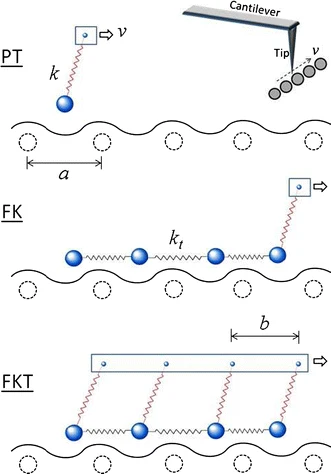
\includegraphics[width=0.4\linewidth]{figures/theory/PT_FK_FKT.png}
  \caption{Illustration of the key features of the Prandtl-Tomlinson (\acrshort{PT}), Frenkel-Kontorova (\acrshort{FK}) and Frenkel-Kontorova-Tomlinson (\acrshort{FKT}) respectively~\cite{Yalin_2011}. \hl{Rights and permissions} \hl{Be careful to align the notation on the figures with the text later on}. \hl{consider to cut up and put side by side.}}
  \label{fig:PT_FK_FKT}
\end{figure}


% Analytical Models for Atomic Friction~\cite{Yalin_2011}
% \textbf{Analytical Models for Atomic Friction}
\subsection{Prandtl–Tomlinson} % Sources for PT model~\cite[2,3]{Yalin_2011} 
The Prandtl–Tomlinson model (\acrshort{PT}) considers a 1D simplification of
the frictional system as a single ball-tip sliding along the rigid substrate as
shown in~\cref{fig:PT_FK_FKT}. The tip is coupled harmonically to a moving support, moving at a constant speed, which drives the tip forward. The interaction between
the tip and the substrate is modeled by a sinusoidal corrugation potential
mimicking the periodicity found in a crystalline substrate. We will consider the
Prandtl–Tomlinson model with added thermal activation as proposed by Gnecco et
al.~\cite{PhysRevLett.84.1172}. For the theoretical foundation of this section,
we generally refer to~\cite{Yalin_2011}. The potential energy for the tip at position $x$ for time $t$ is given as
\begin{align}
  V(x,t) = \frac{1}{2}K(vt - x)^2 - \frac{1}{2}U_0 \cos \left(\frac{2\pi x}{a} \right).
  \label{eq:V_PT}
\end{align}
The first term describes the harmonic coupling with spring constant $K$, between the tip at position $x$ and the moving body at position $vt$, given by its constant speed $v$. The second term describes the corrugation potential with amplitude $U_0$ and period $a$ representing the lattice spacing of the substrate. The dynamics of the tip can be described by the Langevin equations 
\begin{align}
  m \ddot{x}+m \mu \dot{x}=-\frac{\partial V(x, t)}{\partial x}+R(t),
  \label{eq:Langevin_PT}
\end{align}
where $m$ is the mass of the tip, $\mu$ the viscous friction and $R(t)$ the thermal activation term. The equation is solved for tip position $x$ and the friction force is retrieved as the force acting on the moving body
\begin{align*}
  F_{\text{fric}} = K(vt - x).
\end{align*}
The governing equation~\cref{eq:Langevin_PT} belongs to a family of stochastic differential equations composed of both deterministic dynamics and stochastic processes. In this case, the deterministic term is the viscous friction, $m\mu\dot{x}$, to resist the movement of the tip and the force acting from the corrugation potential. The stochastic term is a random force field modeling thermal noise according to the Fluctuation-dissipation relation. Thus, there is no single path but rather multiple paths the tip can take. While the Langevin equation is one of the most common ways to handle thermal activation other methods exist to solve this problem such as Monte Carlo sampling methods. We omit the numerical scheme for the solving of the Langevin equations here and refer instead to a more in-depth discussion of the Langevin equation regarding the \acrshort{MD} simulations in~\cref{sec:langevin}. 


\subsubsection{Thermal activation}
The solving of the Langevin equation, as opposed to Newton's equation of motion, introduces thermal effects to the system. Generally, when the energy barrier comes close to $k_B T$ (\SI{0.026}{eV} at room temperature) thermal effects can not be neglected. In the case of a single asperity contact the energy barrier is on the order \SI{1}{eV} which makes thermal activation significant~\cite{Yalin_2011}. Due to the moving body traveling at a constant speed, the potential energy will increase steadily. Without any temperature, $T = 0$, the slip will only occur when the energy barrier between the current potential well $(i)$ and the adjacent $(j)$ is zero $\Delta V_{i\to j} = 0$. However, in the presence of temperature, we get thermal activation, meaning that the tip can slip to the next potential well sooner at $\Delta V_{i\to j} > 0$. Provided that the sliding speed is slow enough the transition rate $\kappa$ for a slip from the current to the next well is given by
\begin{align}
  \kappa = f_0 e^{-\Delta V / k_B T},
  \label{eq:PT_kappa}
\end{align}
with $\Delta V$ being the energy barrier and $f_0$ the attempt rate. The attempt rate following Kramer’s rate theory~\cite{RevModPhys.62.251} and is related to the mass and damping of the system and can be thought of as the frequency at which the tip ``attempts'' to overcome the barrier. Notice that~\cref{eq:PT_kappa} resembles a microstate probability in the canonical ensemble with $f_0$ in place of the inverse partition function $Z^{-1}$ which provides an additional interpretation of $f_0$. The probability $p_i$ that the tip occupies the current well $(i)$ relative to the adjacent well $(j)$, as illustrated in~\cref{fig:PT_slip} is governed by 
\begin{align}
  \frac{dp_i}{dt} = -\kappa_{i\to j}p_i + \kappa_{j\to i}p_j.
  \label{eq:dpdt_PT}
\end{align}
This probability is related to temperature, speed and mass~\cite{Yalin_2011}.

\begin{figure}[H]
  \centering
  \includegraphics[width=0.6\linewidth]{figures/theory/PT_slip.png}
  \caption{An illustration of slip between two adjacent energy minima. $p_i$ is the probability of the tip residing in the current potential well, $i$, where the energy barrier is $\Delta V_{i \rightarrow j}$. $p_j$ is the probability of the tip residing at the next minima, $j$, where $\Delta V_{j \rightarrow i}$ is the corresponding energy barrier. Figure and caption from~\cite{Yalin_2011}. \hl{Rights and permission}}
  \label{fig:PT_slip}
\end{figure}


Generally, there exist two temperature regimes in the Prandtl–Tomlinson model: The \textit{thermal activation} regime at low temperatures and the \textit{thermal drift} at high temperatures as shown in~\cref{fig:PT_temp}. At lower temperatures, the system is subject to standard thermal activation with a much lower energy barrier for slipping forward than backward $\Delta V_{j \to i} \gg \Delta V_{i \to j}$. This results in a higher transition rate for forward slips, $\kappa_{j \to i} \ll \kappa_{i \to j}$, which effectively inhibits any backward slip. This leads to the simplified expression for~\cref{eq:dpdt_PT}
\begin{align*}
  \frac{dp_i}{dt} = -\kappa_{i\to j}p_i,
\end{align*}
which makes the relationship between friction, temperature and speed follow Sang et al.’s prediction~\cite{Sang_2001}
\begin{align}
  F=F_c-\left|\beta k_B T \ln \left(\frac{v_c}{v}\right)\right|^{2 / 3}, \qquad v_c = \frac{2f_0\beta k_B T}{3 C_{\text{eff}} \sqrt{F_c}},
  \label{eq:F_thermal_ac}
\end{align}
where $F_c$ is the maximum friction at $T = 0$, $v_c$ a critical velocity, $f_0$
is the attempt rate, $c_{eff}$ the effective stiffness, and $\beta$ a
parameter determined by the shape of the corrugation well. \cref{eq:F_thermal_ac} characterizes the decrease in friction with temperature
in the thermal activation regime, shown in~\cref{fig:PT_temp_a} at low temperature. This corresponds with the assumption of only forward slips, as seen in the force trace in~\cref{fig:PT_temp_a}. When the temperature is high enough for the system to be consistently close to thermal equilibrium, it enters the regime of thermal drift~\cite{PhysRevE.71.065101}. This regime transition can be understood through a comparison between two time scales: The time it takes for the moving body to travel one lattice spacing
$t_v = a/v$ and the average time for a slip to occur due to thermal activation
$\tau = 1/\kappa = f^{-1}\exp(\Delta V / k_BT)$. If $t_v \gg \tau$ the system falls within the thermal drift regime, where slips happens both in the forward and backward direction as shown in the force trace in~\cref{fig:PT_temp_b}. For the thermal drift regime, the friction follows the prediction by Krylov et
al.~\cite{Krylow_2007, PhysRevE.71.065101, Jinesh_2008}
\begin{align}
  F \propto \frac{v}{T}e^{1/T}.
  \label{eq:PT_thermal_drift}
\end{align}
Notice that the friction dependence on sliding speed changes from~\cref{eq:F_thermal_ac} to \cref{eq:PT_thermal_drift} as it transitions from the thermal activation to the thermal drift regime. 


\begin{figure}[H]
  \centering
  \begin{subfigure}[t]{0.49\textwidth}
      \centering
      \includegraphics[width=\textwidth]{figures/theory/PT_temp.png}
      \caption{}
      \label{fig:PT_temp_a}
  \end{subfigure}
  \hfill
  \begin{subfigure}[t]{0.49\textwidth}
      \centering
      \includegraphics[width=\textwidth]{figures/theory/PT_temp_force.png}
      \caption{}
      \label{fig:PT_temp_b}
  \end{subfigure}
  \hfill
  \hfill
     \caption{Illustration of the temperature difference between the thermal activation regime and the thermal drift regime. (a) shows the mean friction as a function of temperature showcasing the regime transition. The figure corresponds to the numerical results of Dong et al.~\cite{Yalin_2011} of a Prandtl–Tomlinson model with model parameters: $m=\SI{e-12}{kg}$, $U_0={0.6}{eV}$, $v=\SI{4e3}{nm/s}$, $\mu=\SI{2}{\sqrt{k/m}}$, $a=\SI{0.288}{nm}$. (b) shows the force traces of a simulation in the thermal activation regime (top) and thermal drift regime (bottom) with several characteristic forward and backward slips identified by dashed lines for the latter case. Figures from from~\cite{Yalin_2011} \hl{Rights and permission}.}
     \label{fig:PT_temp}
\end{figure}



\subsubsection{Sliding speed}
In the thermal activation regime (low temperature) and at low sliding speeds, the
friction relation follows~\cref{eq:F_thermal_ac} which means that friction
increases logarithmically with speed. For higher speeds, above the critical
velocity $v > v_c$, if only thermal effects are considered,
\cref{eq:F_thermal_ac} predicts that friction will eventually saturate and come
to a plateau at $F_{\text{fric}} = F_C$. This is illustrated in
\cref{fig:PT_speed} with this prediction being represented by the dotted line.
However, as given away by the figure, for higher speeds the model will enter an
\textit{athermal} regime where the thermal effects are negligible compared to
other contributions~\cite{PhysRevLett.89.224301}. In the athermal regime, the
damping term $m\mu \dot{x}$ will dominate yielding $F_{\text{fric}}\propto v$.
The athermal regime is often observed in reduced-models if the system is
overdamped or at high speeds. This concept is related to \acrshort{MD}
simulations as well where the accessible speeds often fall into the athermal
regime~\cite{Li_2011}. It is unclear how this affects real physical systems for
which there exist more dissipation channels than just a single viscous
term~\cite{Dong_2013}. For the thermal drift regime, at higher temperatures, friction increase linearly with sliding speed $F_{\text{fric}} \propto v$ as given by~\cref{eq:PT_thermal_drift}.

\begin{figure}[H]
  \centering
  \includegraphics[width=0.6\linewidth]{figures/theory/PT_speed.png}
  \caption{The friction dependence on sliding speed for the simulated Prandtl–Tomlinson by Dong et al.~\cite{Yalin_2011} revealing two different regimes. In the thermal regime, friction increases logarithmically with speed, and in the athermal regime, friction is governed by damping such that $F\propto v$. The friction plateau ($F_c = \SI{0.39}{nN}$) predicted by thermal activation is shown as a dotted line. Other models parameters: $m=\SI{e-12}{kg}$, $U_0={0.6}{eV}$, $T = \SI{300}{K}$, $\mu=\SI{2}{\sqrt{k/m}}$, $a=\SI{0.288}{nm}$. Figure from~\cite{Yalin_2011} \hl{Rights and permission}}
  \label{fig:PT_speed}
\end{figure}


\subsubsection{Tip mass}
The mass of the tip affects the dynamics due to a change of inertia, which changes the attempt rate $f_0$. Smaller inertia leads to a larger attempt rate and vice versa. Effectively, this will affect the transition point for the temperature and speed regimes described previously. A smaller inertia, giving a larger attempt rate, will cause an earlier transition (i.e.\ at a lower temperature) to the thermal drift regime. Additionally, this will result in a later speed saturation such that it transitions to the athermal regime at a higher speed. 


\subsubsection{Friction Regimes: Smooth Sliding, Single Slip, and Multiple Slip}
Stick-slip motion is a crucial instability mechanism associated with high energy dissipation and high friction. Thus, controlling the transition between smooth sliding and stick-slip is considered key to controlling friction. We can divide the frictional stick-slip behavior into three regimes: 1) Smooth sliding, where the tip slides smoothly on the substrate. 2) Single slip, where the tip stick at one potential well before jumping one lattice spacing to the next. 3) Multiple slip, where the tip jumps more than one lattice spacing for a slip event. The underlying mechanisms behind these regimes can be understood through static and dynamic contributions. 

To understand the static mechanism we consider a quasistatic process for which temperature, speed and damping can be neglected. For a quasistatic process, we require $\partial(V)/\partial x = 0$. This simplifies~\cref{eq:V_PT} to 
\begin{align}
  \frac{\pi U_0}{a} \sin\left(\frac{2\pi x}{a}\right) \frac{2 \pi}{a} = K(vt - x).
  \label{eq:static_V}
\end{align}
The friction regime is determined by the number of solutions $x$ to~\cref{eq:static_V}. Only one solution corresponds to
smooth sliding, two solutions to a single slip and so on. It turns out that the
regimes can be defined by the parameter $\eta = 2\pi^2U_0/a^2K$~\cite{Johnson_1998, Medyanik_2006} yielding transitions at $\eta = 1, 4.6, 7.79, 10.95, \hdots$, such that $\eta \le 1$
corresponds too smooth sliding, $1<\eta \le 4.6$ to a single slip and so on. These static derivations lay out the fundamental probabilities for being in one of the stick-slip regimes. Notice that increasing the spring constant $K$ (stiff spring) will decrease the possibilities for stick-slip behavior. Similarly, the potential corrugation $U_0$ can be altered by an increasing load~\cite{Vanossi_2013}.

Considering the dynamics on top, one finds that damping, speed and temperature will affect this probability. High damping, equivalent to a high transfer
of kinetic energy to heat, will result in less energy available for the slip events. This will make multiple slip less likely. By a similar argument, we find that increasing the speed will contribute to more kinetic energy which will increase the likelihood of multiple slip. Finally, the temperature will contribute to earlier slips, due to thermal activation, such that
less potential energy can be accumulated and it will result in fewer multiple slip. 

% The effects of damping, speed and temperature are illustrated for the force traces in~\cref{fig:PT_slip_var}


% \begin{figure}[H]
%   \centering
%   \begin{subfigure}[t]{0.32\textwidth}
%       \centering
%       \includegraphics[width=\textwidth]{figures/theory/PT_slip_damping.png}
%       \caption{}
%   \end{subfigure}
%   \hfill
%   \begin{subfigure}[t]{0.32\textwidth}
%       \centering
%       \includegraphics[width=\textwidth]{figures/theory/PT_slip_speed.png}
%       \label{fig:PT_slip_vel}
%       \caption{}
%   \end{subfigure}
%   \hfill
%   \begin{subfigure}[t]{0.32\textwidth}
%       \centering
%       \includegraphics[width=\textwidth]{figures/theory/PT_slip_temp.png}
%       \caption{}
%   \end{subfigure}
%   \hfill
%      \caption{\hl{Temporary} figure from~\cite{Yalin_2011}. \hl{Consider removing since the interpretation of smooth sliding might get a bit tricky.}}
%      \label{fig:PT_slip_var}
% \end{figure}



% Together with the current experimental possibility to perform well-defined
% measurements on well-characterized materials at the fundamental microscopic
% level of investigation of the sliding contacts, advances in the computer
% modeling of interatomic interactions in materials science and complex systems
% encompass molecular-dynamics (MD) simulations of medium to large scale for the
% exploration of the tribo-dynamics with atomic resolution [4, 5].




\subsection{Frenkel-Kontorova}
% Based on~\cite{Manini_2016} and~\cite{FK2D}.
The Frenkel-Kontorova (\acrshort{FK}) model~\cite{Frenkel_1938} extends the Prandtl–Tomlinson model by considering a chain of atoms in contrast to just a single particle (tip). This extension is useful for understanding the importance of the alignment between the atoms and the substrate, the so-called \textit{commensurability}. Our review of the Frenkel-Kontorova is based on~\cite{Manini_2016, Vanossi_2013}.

The standard Frenkel-Kontorova model consists of a 1D chain of $N$ classical particles of equal mass, representing atoms, interacting via harmonic forces and moving in a sinusoidal potential as sketched in~\cref{fig:FK_model}~\cite{Manini_2016}. The Hamiltonian is 
\begin{align}
  H = \sum_{i=1}^N \left[\frac{p_i^2}{2m} + \frac{1}{2}K(x_{i+1} - x_i - a_c)^2 + \frac{1}{2}U_0 \cos{\left(\frac{2\pi x_i}{a_b}\right)}\right],
  \label{eq:H_FK}
\end{align}
where the atoms are labelled sequently $i = 1, \hdots, N$. The first term $p_i^2/2m$ represents the kinetic energy with momentum $p_i$
and mass $m$. Often the effects of inertia are neglected, referred to as the static Frenkel-Kontorova model, while the inclusion in‘\cref{eq:H_FK} is known as the dynamic Frenkel-Kontorova model~\cite{FK2D}. The next term describes the harmonic interaction with elastic
constant $K$, nearest neighbor distance $\Delta x = x_{i+1} - x_i$ and 
corresponding nearest neighbor equilibrium distance $a_c$. The final term represents the periodic corrugation potential, with amplitude $U_0$ and period $a_b$. By comparison to the potential used in the Prandtl–Tomlinson model \cref{eq:V_PT}, the difference is the introduction of a harmonic coupling between particles in the chain as opposed to the moving body. Different boundary choices can be made where both free ends and periodic conditions give similar results. The choice of fixed ends however makes the chain incapable of sliding.

\begin{figure}[H]
  \centering
  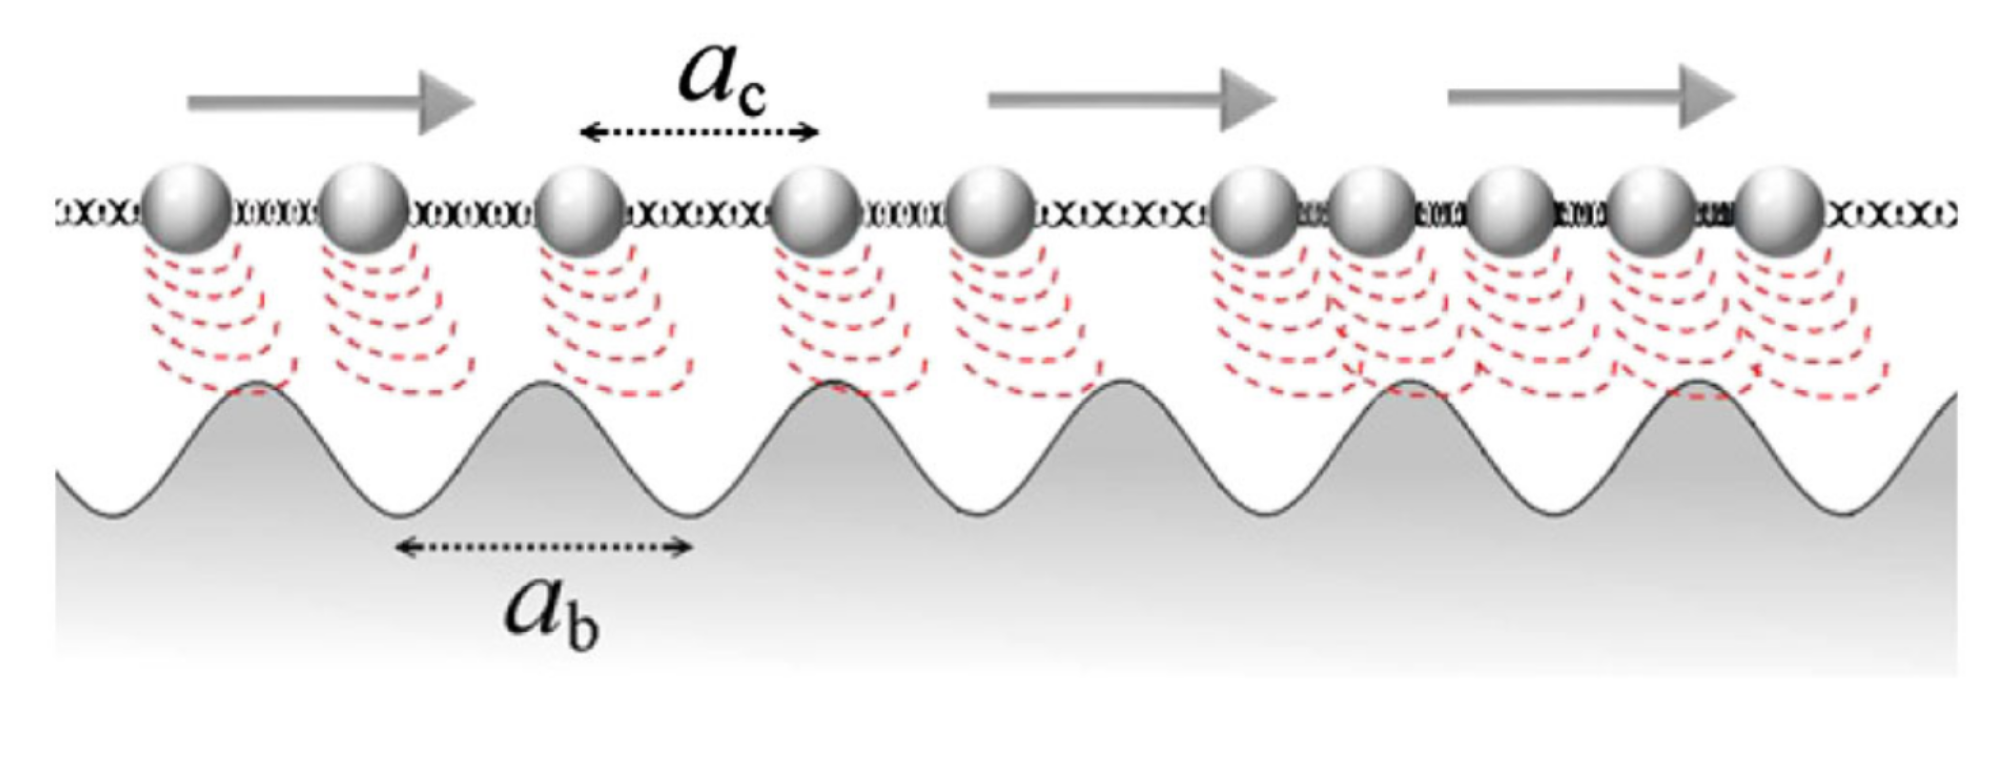
\includegraphics[width=0.8\linewidth]{figures/theory/FK_model.png}
  \caption{\hl{Waiting for reuse permission} figure from~\cite{Manini_2016}}
  % https://powerxeditor.aptaracorp.com/sciprisaps/RnPRequest/List
  \label{fig:FK_model}
\end{figure}

To probe static friction one can apply an external adiabatically increasing force until sliding occurs, i.e.\ without loss or gain of heat. This corresponds to the static Frenkel-Kontorova model, and it turns out that the sliding properties are entirely governed by its topological excitations referred to as so-called \textit{kinks} and \textit{antikinks}

\subsubsection{Commensurability} We can subdivide the frictional behavior in terms of commensurability, that is, how well the spacing of the atoms matches the periodic substrate potential. We describe this by the length ratio $\theta = a_b / a_c = N / M$ where $M$ denotes the number of minima in the potential within the length of the chain. A rational number for $\theta$ means that we can achieve a perfect alignment between the atoms in the chain and the potential minima, without stretching the chain, corresponding to a \textit{commensurate} case. If $\theta$ is irrational the chain and substrate cannot fully align without some stretching of the chain, and we denote this as being \textit{incommensurate}.

We begin with the simplest commensurate case of $\theta = 1$ where the spacing
of the atoms matches perfectly with the substrate potential periodicity, i.e.\
$a_c = a_b$, $N = M$. The ground state (\acrshort{GS}) is the configuration
where each atom is aligned with one of the substrate minima. By adding an extra
atom to the chain we would effectively shift some of the atoms, out of this
ideal state, giving rise to a kink excitation. This leads to the case where two
atoms will have to ``share'' the same potential corrugation as sketched in
\cref{fig:incommensurable_example}. On the other hand, removing an atom from
the chain results in an antikink excitation where one potential corrugation will
be left ``atomless''. In order to reach a local minimum the kink (antikink) will
expand in space over a finite length such that the chain undertakes a local
compression (expansion). Notice that for low ratios of $\theta$, fewer atoms than minima, the chain will not be able to fill each corrugation well in any case. In this case, commensurability can instead be thought of as whether the atoms are forced to deviate, by a lattice spacing, from the spacing otherwise dictated by the spring forces in-between. When applying a tangential force to the chain it is much
easier for an excitation to move along the chain than it is for the non-excited
atoms since the activation energy for a kink/antikink
displacement is systematically smaller (often much smaller) than the potential
barrier $U_0$. Thus, the motion of kinks (antikinks), i.e.\ the displacement of
extra atoms (atom vacancies), is representing the fundamental mechanism for
mass transport. These displacements are responsible for the mobility,
diffusivity and conductivity within this model. 

In the zero temperature commensurable case with an adiabatical increase in force, all atoms would be put into an accelerating motion as soon as the potential barrier energy is present. However, similar to our discussion on the Prandtl-Tomlinson model, thermal activations will excite the system at an earlier stage resulting in kink-antikink pairs traveling down the chain. For a chain of finite length, these often occur at the end of the chain running in opposite directions. This cascade of kink-antikink excitations is shown in \cref{fig:kink_antikink}. Notice, that for the 2D case, where an island (flake) is deposited on a surface, we generally also expect the sliding to be initiated by kink-antikink pairs at the boundaries. 


\begin{figure}[H]
  \centering
  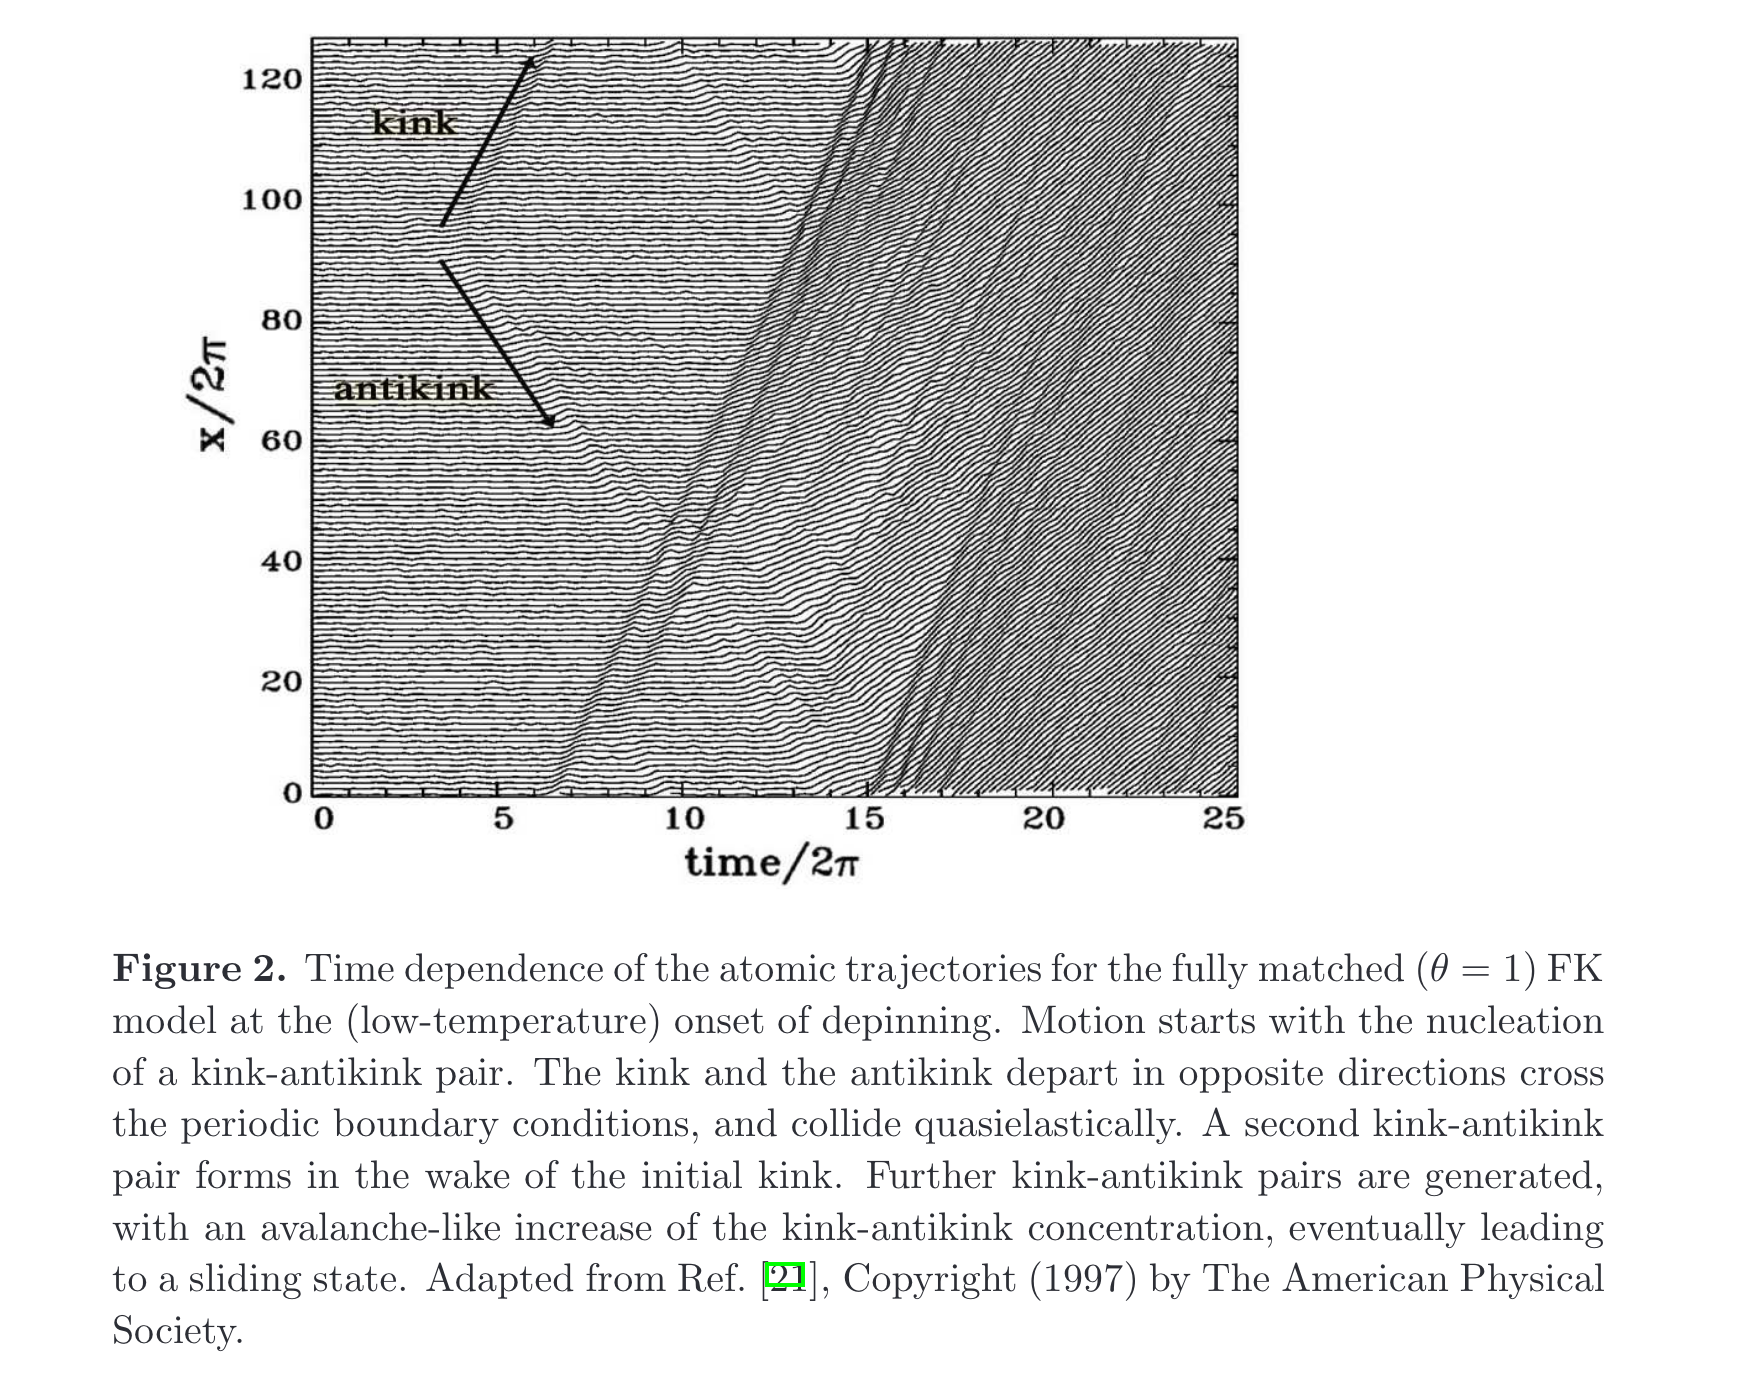
\includegraphics[width=0.8\linewidth]{figures/theory/kink_antikink.png}
  \caption{\hl{Waiting for reuse permission} figure from~\cite{Manini_2016}}
  % https://powerxeditor.aptaracorp.com/sciprisaps/RnPRequest/List
  \label{fig:kink_antikink}
\end{figure}


% where the chain is slightly compressed (expanded) to match the substrate potential, separated by kinks (antikinks), where the increased stress is eventually released.
% as illustrated in \cref{fig:incommensurable_example} 
% through a localized expansion (compression) 

% \hl{Go through this last part  again. Even though this is what the source says I'm not quite sure I understand why it is not opposite ``...released through a localized compression (expansion)''?}.

\begin{figure}[H]
  \centering
  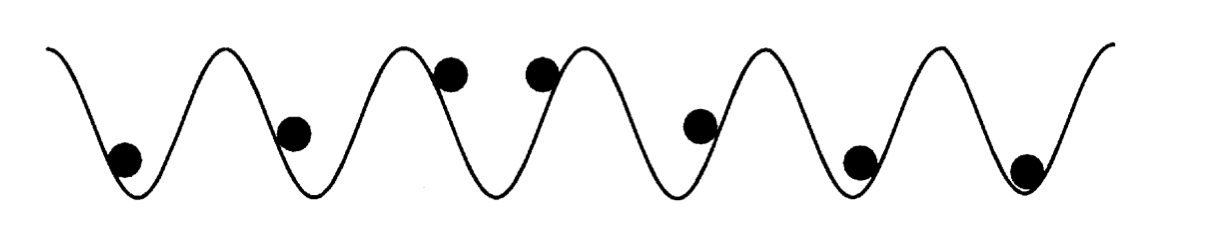
\includegraphics[width=0.5\linewidth]{figures/theory/incommensurable_example.png}
  \caption{\hl{Temporary} figure from
  url{http://www.iop.kiev.ua/~obraun/myreprints/surveyfk.pdf} p. 14.
  Incommensurable case ($\theta = ?$) where atoms sits slightly closer than
  otherwise dictated by the substrate potential for which this regular result in
  a kink here seen as the presence of two atoms closely together in one of the
  potential corrugations.}
  \label{fig:incommensurable_example}
\end{figure}

% Maybe use the strength $\lambda = U_0 / (K a_b^2)$ with critical strength $\lambda_c$ instead of critical $K$?

For the case of incommensurability, i.e.\ $\theta = a_b/a_c$ being irrational, the
\acrshort{GS} is characterized by a sort of ``staircase''  deformation. That is, the chain will exhibit regular periods of regions with approximate commensurability separated by reguraly spaced kinks or antikinks. 


The incommensurable Frenkel-Kontorova model contains a critical elastic constant $K_c$, such that for $K > K_c$ the static friction $F_s$ drops to zero, making the chain able to initiate a slide at no energy cost, while the low-velocity kinetic friction is dramatically reduced. This can be explained by the
fact that the displacement occurring in the incommensurable case will yield just
as many atoms climbing up a corrugation as atoms climbing down. For a big (infinite) chain this will exactly balance the forces making it
non-resistant to sliding. Generally, incommensurability guarantees that the
total energy (at $T=0$) is independent of the relative position to the
potential. However, when sliding freely, a single atom will eventually occupy a
maximum of the potential, and thus when increasing the potential magnitude $U_0$ or
softening the chain stiffness, lowering $K$, the possibility to occupy such a
maximum disappears. This marks the so-called \text{aubry transition},
at the critical elastic constant $K = K_c(U_0, \theta)$, where the chain goes
from a free sliding to a \textit{pinned} state with nonzero static friction.
$K_c$ is a discontinuous function of the ratio $\theta$, due to the reliance on
irrational numbers for incommensurability. The minimal
value $K_c \simeq 1.0291926 $ in units $[2 U_0 (\pi / a_b)^2]$ is achieved for
the golden-mean ratio $\theta = (1+\sqrt{5}/2)$. The Aubry transition can be investigated as a first-order phase transition for which power laws can be defined for the order parameter, but this is beyond the scope of this thesis.


% The term superlubricity has been criticized as mislead-
% ing, since it might wrongly suggest zero friction in the sliding state in analogy to superconductivity and super- fluidity. Instead, incommensurability of periodic inter- faces cancels only one of the channels of energy dissipa- tion, that originating from the low-speed stick-slip insta- bility. Other dissipative processes, such as the emission of sound waves, still persist, and therefore even in the case of complete incommensurability the net kinetic friction force does not vanish. Nonetheless, in the superlubric regime one expects a substantial reduction of the friction force relative to a similar, but commensurate case.
% https://arxiv.org/abs/1112.3234v4


The phenomena of non-pinned configurations are named \textit{superlubricity} in
tribological context. Despite the misleading name, this refers to the case
where the static friction is zero while the kinetic friction is nonzero, but
reduced. For the case of a 2D sheet, it is possible to alter the
commensurability, not only by changing the lattice spacing through material
choice but also by changing the orientation of the sheet relative to the
substrate. Dienwiebel et al.~\cite{DIENWIEBEL2005197} have shown that the
kinetic friction, for a graphene flake sliding over a graphite surface (multiple
layers of graphene), exhibits extremely low friction at certain orientations as
shown in \cref{fig:graphene_rot}. As the orientation is changed they observed two spikes of considerable friction while the remaining valleys correspond to effectively zero friction in consideration of the measurement uncertainty. This phenomenon relates to the transition between frictional regimes, as introduced through the Prandtl–Tomlinson model, since the change in orientation affects the
effective substrate potential. Merely from the static consideration, we found that
lowering the potential amplitude $U_0$ will decrease the parameter $\eta =
2\pi^2U_0/a^2K$ shifting away from the regime of multiple slips towards smooth
sliding associated with low friction. Such transitions will also be affected by the shape of the potential and corresponding 2D effects of the sliding path~\cite{Yalin_2011}.

\begin{figure}[H]
  \centering
  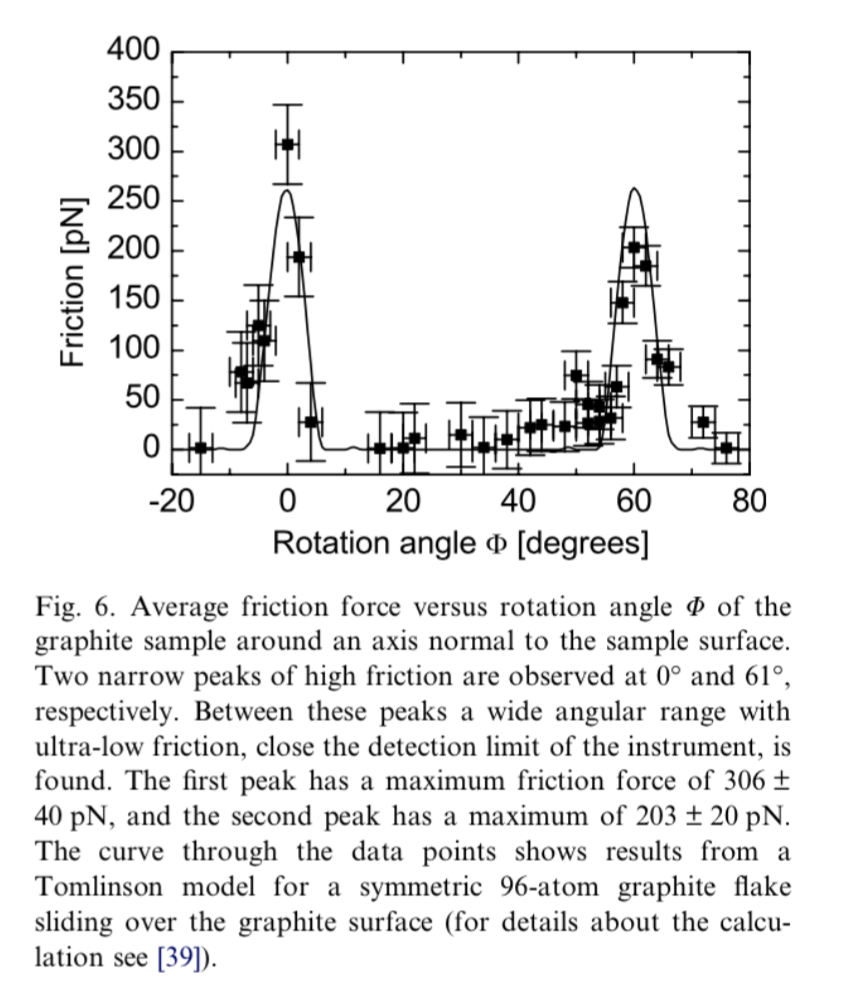
\includegraphics[width=0.5\linewidth]{figures/theory/graphene_rot.png}
  \caption{\hl{Temporary} figure from~\cite{DIENWIEBEL2005197} showing superlubricity for incommensurable orientations between graphene and graphite. \hl{temporary}}
  \label{fig:graphene_rot}
\end{figure}




% The reason that friction lowers for incommensurability is 
% probably that we avoid stick-slip behavior which is highly 
% ``strongly dissipative stick-slip motion''~\cite{bonelli_atomistic_2009}


% Maybe check out for more info on the 1D model: Y. S. Kivshar O. M. Braun. The Frenkel-Kontorova Model. Springer, 1st edition, 2004.
% The Frenkel-Kontorova Model.pdf p. 38 3.2 Dynamics of Kinks <---------

%Based on~\cite{FK2D}


% The Frenkel-Kontorova model can also describe phonons and heat in the lattices, which absorb the kinetic energy of the sliding[4].~\cite{FK2D}

% Consequently, the Frenkel-Kontorova model is the simplest model in which dynamic friction is emergent, while in other models some form of heuristic damping must be included.\cite{FK2D}
\subsubsection{Velocity resosnance} % Velocity resosnance 
% The kinetic friction properties of the FK model (Strunz and Elmer, 1998a,b) are probed by adding a (e.g. Langevin) thermostat as described for the PT model above. Even where (above the Aubry transition) Fs = 0 the kinetic friction force Fk is nonzero, because the dy- namics at any finite speed results in the excitation of phonons in the chain.
% https://arxiv.org/abs/1112.3234v4

While many of the same arguments used for the Prandtl–Tomlinson model regarding velocity dependence for friction can be made for the Frenkel-Kontorova model, the addition of multiple atoms introduces the possibility of resonance. In the Frenkel-Kontorova model, the kinetic friction is primarily attributed to resonance between the sliding-induced vibrations and phonon modes in the chain~\cite{FK2D}. The specific dynamics are found to be highly model and dimension specific, and even for the 1D case, this is rather complex. However, we make a simplified analysis of the 1D rigid chain in order to showcase the reasoning behind the phenomena.

When all atoms are sliding rigidly with center of mass (\acrshort{CM}) velocity $v_{{\text{CM}}}$ the atoms will pass the potential maxima with the so-called \textit{washboard frequency} $\Omega = 2\pi v_{{\text{CM}}} / a_b$. For a weak coupling between the chain and the potential we can use the zero potential case as an approximation for which the known dispersion relation for the 1D harmonic chain is given~\cite[p. 92]{Kittel2004}
\begin{align*}
  \omega_k = \sqrt{\frac{4 K}{m}} \left|\sin{\left(\frac{k}{2}\right)}\right|,
\end{align*}
where $\omega_k$ is the phonon frequency and $k = 2\pi i / N$ the wavenumber with $i\in [N/2, N/2)$. Resonance will occur when the washboard frequency $\Omega$ is close to the frequency of the phonon modes $\omega_q$ in the chain with wavenumber $q = 2\pi a_c / a_b = 2\pi \theta^{-1}$ or its harmonics $nq$ for $n = 1, 2, 3, \hdots$~\cite{van_den_Ende_2012}. Thus, we can approximate the resonance \acrshort{CM} speed as
\begin{align*}
    n \Omega &\sim \omega_{nq} \\
    n \frac{2\pi v_{\text{CM}}}{a_b} &\sim \sqrt{\frac{4K}{m}} \left| \sin{\left(\frac{2n \pi \theta^{-1}}{2}\right)}\right| \\
    v_{\text{CM}} &\sim \frac{\sin{(n\pi \theta^{-1})}}{n \pi} \sqrt{\frac{Ka_b^2}{m}}.
\end{align*}
When the chain slides with a velocity around resonance speed, the washboard
frequency can excite acoustic phonons which will dissipate to other phonon modes
as well. At zero temperature, the energy will transform back and forth between
internal degrees of freedom and \acrshort{CM} movement of the chain. Without any dissipation mechanism, this is theorized to speed up the translational decay~\cite{FK2D}. However, as soon as we add a dissipation channel through the substrate, energy will dissipate from the chain to the substrate's degrees of freedom. This suggests that certain sliding speeds will exhibit relatively high kinetic friction while
others will be subject to relatively low kinetic friction. Simulations of
concentric nanotubes in relative motion (telescopic sliding) support this idea
as it has revealed the occurrence of certain velocities at which the friction is
enhanced, corresponding to the washboard frequency of the
system~\cite{Zhang_2007, Zhang_2009}. The friction response was observed to be highly non-linear as the resonance velocities were approached. 

The analysis of the phonon dynamics is highly simplified here, and a numerical study of the Frenkel-Kontorova by Norell et al.~\cite{FK2D} showed that the behavior was highly dependent on model parameter choices, but that the friction generally increased with velocity and temperature. Here the latter observation differs qualitatively from that of the Prandtl–Tomlinson model.



% This is strongly connected to the superlubricity term, although the phonon
% dynamics in this analysis is overly simplified, and additionaly we expect more
% complex resonance dynamics for higher dimensions. 


% A common way to model the non-zero temperature case is by the use of a Langevin
% thermostat, which models the dissipation of heat by adding a viscous damping
% force and thermal fluctuations by the addition of Gaussian random forces with
% variance proportional to the temperature (see \cref{sec:langevin} for more details). In combination, this gives rise to a kinetic
% friction that is both velocity and temperature dependent. By extending the Frenkel-Kontorova model into 2D~\cite{FK2D} it can be shown numerically that
% the friction coefficient generally increases with increasing velocity and
% temperature resepectively, although the specific of the trend is highly
% sensitive to model parameters. 




% As the system is Hamiltonian (no heuristic damping) the total energy is conserved. Nevertheless, energy can be transferred from the centre of mass to the internal degrees of freedom, leading to the arrest of the chain in time. This effect can be interpreted as an effective friction.~\cite{van_den_Ende_2012}


% The majority [6–12] examines the steady state of the dynamical Frenkel-Kontorova model in the presence of dissipation, rep- resenting the coupling of phonons to other, undescribed degrees of freedom.~\cite{PhysRevLett.85.302}


% Static friciton behvaiour is robust and remains similar in 2D but dynamical friction is strongly influenced. 




% When considering the nonzero temperature thermal fluctuations can then overcome pinning effects even in fully commensurate cases.



% By applying a finite driving force it is known that a pinned configuration will go through several first-order dynamical pahse transitions as the system transfers from a pinned to a sliding state. 



% At face value, the transition from a static strained configuration to full
% sliding is conceptually as simple as overcoming an energy barrier. However,
% practical single- and multiple- contact conditions are characterized by
% complex interaction profiles plus nontrivial internal dynamics. As a result,
% the interplay of thermal drifts, contact ageing, contact-contact in-
% teractions, and macroscopic elastic deformations introduce significant
% complications, and make the depinning transition from static to kinetic
% friction an active field of research. The depinning dynamics affects in
% particular the transition between stick-slip and smooth slid- ing for sliding
% friction. (Current trends in the physics of nanoscale friction)


% In Atomic Force Microscopy (AFM) experiments, when the tip scans over the
% monolayers at low speeds, friction force is reported to increase with the
% logarithm of the velocity, similar to that observed when the tip scans across
% crystalline surfaces. This velocity dependence is interpreted in terms of
% thermally activated depinning of interlocking barriers involving interfacial
% atoms. (Current trends in the physics of nanoscale friction)






% "However, it is well known that continuum mechanics is valid only when the dimensions of the studied object are much larger than the length scale of the atomic disconti- nuity. Therefore, when the scale of the single asperity is on the order of nanometers, the effect of the discontinuity of the atoms within the tip and substrate can no longer be neglected [47]. Recent AFM experiments on metals revealed that friction varies little with increase of normal load in the low load regime [24, 74]. In addition, a newly invented AFM technique referred to as tip-on-top mode that enables researchers to manipulate nanoparticles of different size showed that in some cases friction increased linearly with interface area while in other cases near fric- tionless sliding was observed [75]. These conflicting results suggest that there may be a non-linear relationship between real contact area and friction."~\cite{Yalin_2011}


% The essential difference between the FK and FKT models is that only the end atom is attached to the support in FK while all atoms are attached to the support in FKT.~\cite{Yalin_2011}


% The friction comes from the viscous force which is proportional to sliding speed. Physically speaking, the viscous term is due to phonon excitation. So the term ‘‘superlubricity’’ which suggests cancelation of friction to zero may not be appropriate; structural lubricity proposed by Mu ̈ser is a better term to describe the phenomenon [77].~\cite{Yalin_2011}



\subsection{Frenkel-Kontorova-Tomlinson}
A final extension of the atomic models worth mentioning here is the
Frenkel-Kontorova-Tomlinson (\acrshort{FKT}) model~\cite{weiss_dry_1997}, which
introduces a harmonic coupling of the sliding atom chain to the moving body,
effectively combining Prandtl–Tomlinson and Frenkel-Kontorova
(see~\cref{fig:PT_FK_FKT}). This introduces more degrees of freedom to the model
which is based on the intention of getting a more realistic connection between
the moving body and the chain. Dong et al.~\cite{Yalin_2011} carried out a numerical analysis
using the 1D Frenkel-Kontorova-Tomlinson model to investigate the effect of
chain length. They observed that the friction increased linearly with the number
of atoms in the chain on a long range, but certain lattice mismatches resulted in
local non-linear relationships as shown in~\cref{fig:FKT_contact}. Similarly, by
extending the Frenkel-Kontorova-Tomlinson model to 2D they were able to achieve
a similar sensitivity to commensurability as observed experimentally
by~\cite{DIENWIEBEL2005197} (see ~\cref{fig:graphene_rot}) with the numerical
result shown in~\cref{fig:FKT_2D_rot}. Besides a demonstration of the
commensurability effect in 2D they also observed increasing friction with an
increasing flake size. Combined, the 1D and 2D results support the idea of
increasing friction with contact size although it might showcase non-linear
behavior depending on commensurability.


\begin{figure}[H]
  \centering
  \begin{subfigure}[t]{0.49\textwidth}
      \centering
      \includegraphics[width=\textwidth]{figures/theory/FKT_contact.png}
      \label{fig:FKT_contact}
  \end{subfigure}
  \hfill
  \begin{subfigure}[t]{0.49\textwidth}
      \centering
      \includegraphics[width=\textwidth]{figures/theory/FKT_2D_rot.png}
      \label{fig:FKT_2D_rot}
    \end{subfigure}
    \hfill
     \caption{Friction in the Frenkel-Kontorova-Tomlinson model for varying size and Commensurability corresponding to numerical result by Dong et al.~\cite{Yalin_2011}. $K_t$ describes the interatomic spring constant and $K$ the coupling to the moving body. (a) The 1D case with an increasing number of atoms in the chain and different mismatch length ratios $\theta = a_b / a_c$, given as $a/b$ in their notation. The model parameters are $K = \SI{5}{N/m}$, $K_t = \SI{50}{N/m}$. (b) The 2D case with varying angles (misfit angle) between the flake and the substrate. The model parameters are $K = \SI{10}{N/m}$, $K_t = \SI{50}{N/m}$. Figure from~\cite{Yalin_2011}. \hl{Rights and permission}.}
     \label{fig:FKT_size}
\end{figure}


\subsection{Shortcomings of reduced-models}
On a final note, we point out that the reduced-models describe the friction behavior in a highly simplified manner. Some shortcomings include the fact that they assume a rigid substrate with a simple sinusoidal potential shape. In reality, the substrate reaction to sliding motion will make for a changing potential throughout the simulation which makes the dynamics more complex. Similarly, the energy dissipation is simplified through a viscous term $-m\mu \dot{x}$ from the Langevin equations \cref{eq:Langevin_PT}. This does not capture the full complexity associated with electron and phonon dissipation~\cite{Yalin_2011}. Taking phonon dissipation as an example there are $3N$ vibration modes, and thus many dissipation channels for the tip. Finally, we also point out that the moving body is simplified as a constantly moving rigid body, while in reality, this might also be subject to more complex dynamic behavior.



% \hl{To-DO: Shortcomings of PT-based reduced-models} %~\cite{Yalin_2011}. 
% \begin{itemize}
%   \item Assumes a rigid substrate with a simplified potential shape. 
%   \item Energy dissipation is added through a viscous term $-m\mu \dot{x}$ being the only dissipation channel availble. Does not capture a more complex real-life electron and phonon dissipation. Taking phonon dissipation as an example there are many vibration modes (3N). This will affect the thermal activation derivation. 
%   \item The moving body is simplified as a constantly moving rigid body, while in fact this will also be subject to a more complex dynamic behavior.
% \end{itemize}


% However, Weiss and Elmer (1995) proposed that the model had a deficiency. They suggested that in the FK model, there was no connection between the atoms and the sliding body. Therefore, Frenkel-Kontorova-Tomlinson (FKT) model that combines the FK model with the Tomlinson model was proposed.~\cite{kim_nano-scale_2009}


% The Frenkel-Kontorova-Tomlinson (FKT) model [61, 62] introduces an harmonic
% coupling of the sliding atomic chain to a driving moving body, thus making it
% possible to investigate stick-slip features in a 1D extended simplified
% contact. The FKT framework provided the ideal platform to investigate the
% tribological consequences of combined interface incommensurability,
% finite-size effects, mechanical stiffness of the contacting materials, and
% normal-load variations~\cite{Manini_2016}.


% Important generalizations involving increased dimensionality compared to the
% regular FK model bear significant implications for tribological properties
% such as critical exponents, size-scaling of the friction force, depinning
% mechanisms, and others.~\cite{Manini_2016}

% Maybe check this out: An interesting example of such a transient is the
% depinning of an atomic monolayer driven across a 2D periodic substrate profile
% of hexagonal symmetry [83]. ~\cite{Manini_2016}


% \subsection{Other stuff}


% At nanoscales things get a bit more unclear. SFM (explain) experiments have
% reported (copy sources 5, 6, 21 from~\cite{mo_friction_2009}) where $F_f \propto
% F_N$ or even with these quantities being nearly independent of each other.

%~\cite{physicsworld_2005}

% Physically relevant quantities, including the average friction force, the slider and the lubricant mean velocities, several correlation functions, and the heat flow can be evaluated numerically by carrying out suitable averages over the model dynamics of a sliding interface, as long as it is followed for a sufficiently long time. The modeling of friction must first of all address correctly ordinary equilibrium and near-equilibrium phenomena, where the fluctuation-dissipation theorem (Sec. 2) governs the smooth conversion of mechanical energy into heat, but most importantly it must also deal with inherently nonlinear dissipative phenomena such as instabilities, stick-slip, and all kinds of hysteretic response to external driving forces, characteristic of non-equilibrium dynamics. 
%~\cite{Manini_2016}


% In several works by J. Fineberg’s group [2–4] the transition from sticking to
% sliding is characterized by slip fronts propagating along the interface.
%~\cite{Manini_2017}[p. 2]. 



% As expected, high levels of
% friction were present in the commensurate positions and extremely low friction
% was found when the surfaces were incommensurate.
% (\url{https://physicsworld.com/a/friction-at-the-nano-scale/})


% Superlubricity, now a pervasive concept of
% modern tribology, dates back to the math- ematical framework of the Frenkel
% Kontorova model for incommensurate interfaces [40]. When two contacting
% crystalline workpieces are out of registry, by lattice mismatch or angular
% misalignment, the minimal force required to achieve sliding, i.e. the static
% friction, tends to zero in the thermodynamic limit – that is, it can at most
% grow as a power less than one of the area – provided the two substrates are
% stiff enough. (Current trends in the physics of nanoscale friction)


% Superlubricity is experimentally rare. Until recently, it has been
% demonstrated or im- plied in a relatively small number of cases [29, 42–46].
% There are now more evidences of superlubric behavior in cluster
% nanomanipulation [32, 33, 47], sliding colloidal layers [48–50], and
% inertially driven rare-gas adsorbates [51, 52]. (Current trends in the physics
% of nanoscale friction)


% A breakdown of structural lubricity may occur at the heterogeneous interface
% of graphene and h-BN. Because of lattice mismatch (1.8\%), this interface is
% intrinsically incommen- surate, and superlubricity should persist regardless
% of the flake-substrate orientation, and become more and more evident as the
% flake size increases [57]. However, vertical cor- rugations and planar strains
% may occur at the interface even in the presence of weak van der Waals
% interactions and, since the lattice mismatch is small, the system can de-
% velop locally commensurate and incommensurate domains as a function of the
% misfit angle [58, 59]. Nonetheless, spontaneous rotation of large graphene
% flakes on h-BN is observed after thermal annealing at elevated temperatures,
% indicative of very low friction due to incommensurate sliding [60, 61].
% (Current trends in the physics of nanoscale friction)

% Indeed, we know from theory and simulation [74–76] that even in clean wearless
% friction experiments with perfect atomic structures, superlubricity at large
% scales may, for example, surrender due to the soft elastic strain deformations
% of contacting systems. (Current trends in the physics of nanoscale friction)



% \section{Multi scale models?}
%~\cite{Manini_2016} p. 24.


% Might find something interesting here~\cite{zhao_thermally_2007} or~\cite{PhysRevE.71.065101}.

% Find a suitable place to introduce smooth sliding. Above certain velocities the stick-slip motion dissapear.~\cite[p. 142-ish]{gnecco_meyer_2015}

\subsection{Experimental procedures}
%~\cite{gnecco_meyer_2015}
% Check out this~\cite{Dong_2013} parameter choices for MD

Experimentally, the study of nanoscale friction is challenging due to the low
forces on the scale of nano-newtons along with the difficulties of mapping the
nano-scale topography of the sample. In contrast to numerical simulations, which provide full
transparency regarding atomic-scale structures, sampling of forces, velocities
and temperature, the experimental results are limited by the state-of-the-art
experimental methods. To compare numerical and experimental results we adress a few of the most relevamt experimental methods.

\subsubsection{Scanning Probe Microscopy}\label{sec:SPM} Scanning probe
microscopy (\acrshort{SPM}) includes a variety of experimental methods which is
used to examine surfaces with atomic resolution~\cite[pp.
6-27]{BHUSHAN20051507}. This was originally developed for surface topography
imaging, but today it plays a crucial role in nanoscale science as it is used
for probe-sampling regarding tribological, electronic, magnetic, biological and
chemical character. The family of methods involving the measurement of forces is
generally referred to as \textit{scanning force microscopies} (\acrshort{SFM})
or for friction purposes \textit{friction force microscopes} (\acrshort{FFM}).

One such method arose from the \textit{atomic force microscope} \acrshort{AFM}, which consists of a sharp micro-fabricated tip attached to a cantilever force sensor, usually with a sensitivity below 1 nN all the way down to pN. The force is measured by recording the bending of
the cantilever, either as a change in electrical conduction or more commonly, by
a light beam reflected from the back of the cantilever into a photodetector
\cite[p. 183]{gnecco_meyer_2015}. By adjusting the tip-sample height to keep a constant normal force while scanning across the surface, the \acrshort{AFM} can be used to produce a
surface topography map. By tapping the material (dynamic force microscopy) with
a sinusoidally vibrated tip the effects from friction and other disturbing forces
can be minimized to produce an even clearer image (\hl{include example,
preferably showing the surface structure of graphene}). However, when scanning
perpendicularly to the cantilever axis, one is also able to measure the
frictional force as torsion of the cantilever. By having four quadrants in the
photodetector (as shown in figure \cref{fig:AFM}), one can simultaneously
measure the normal force and friction force as the probes scan across the
surface. 

\begin{figure}[H]
  \centering
  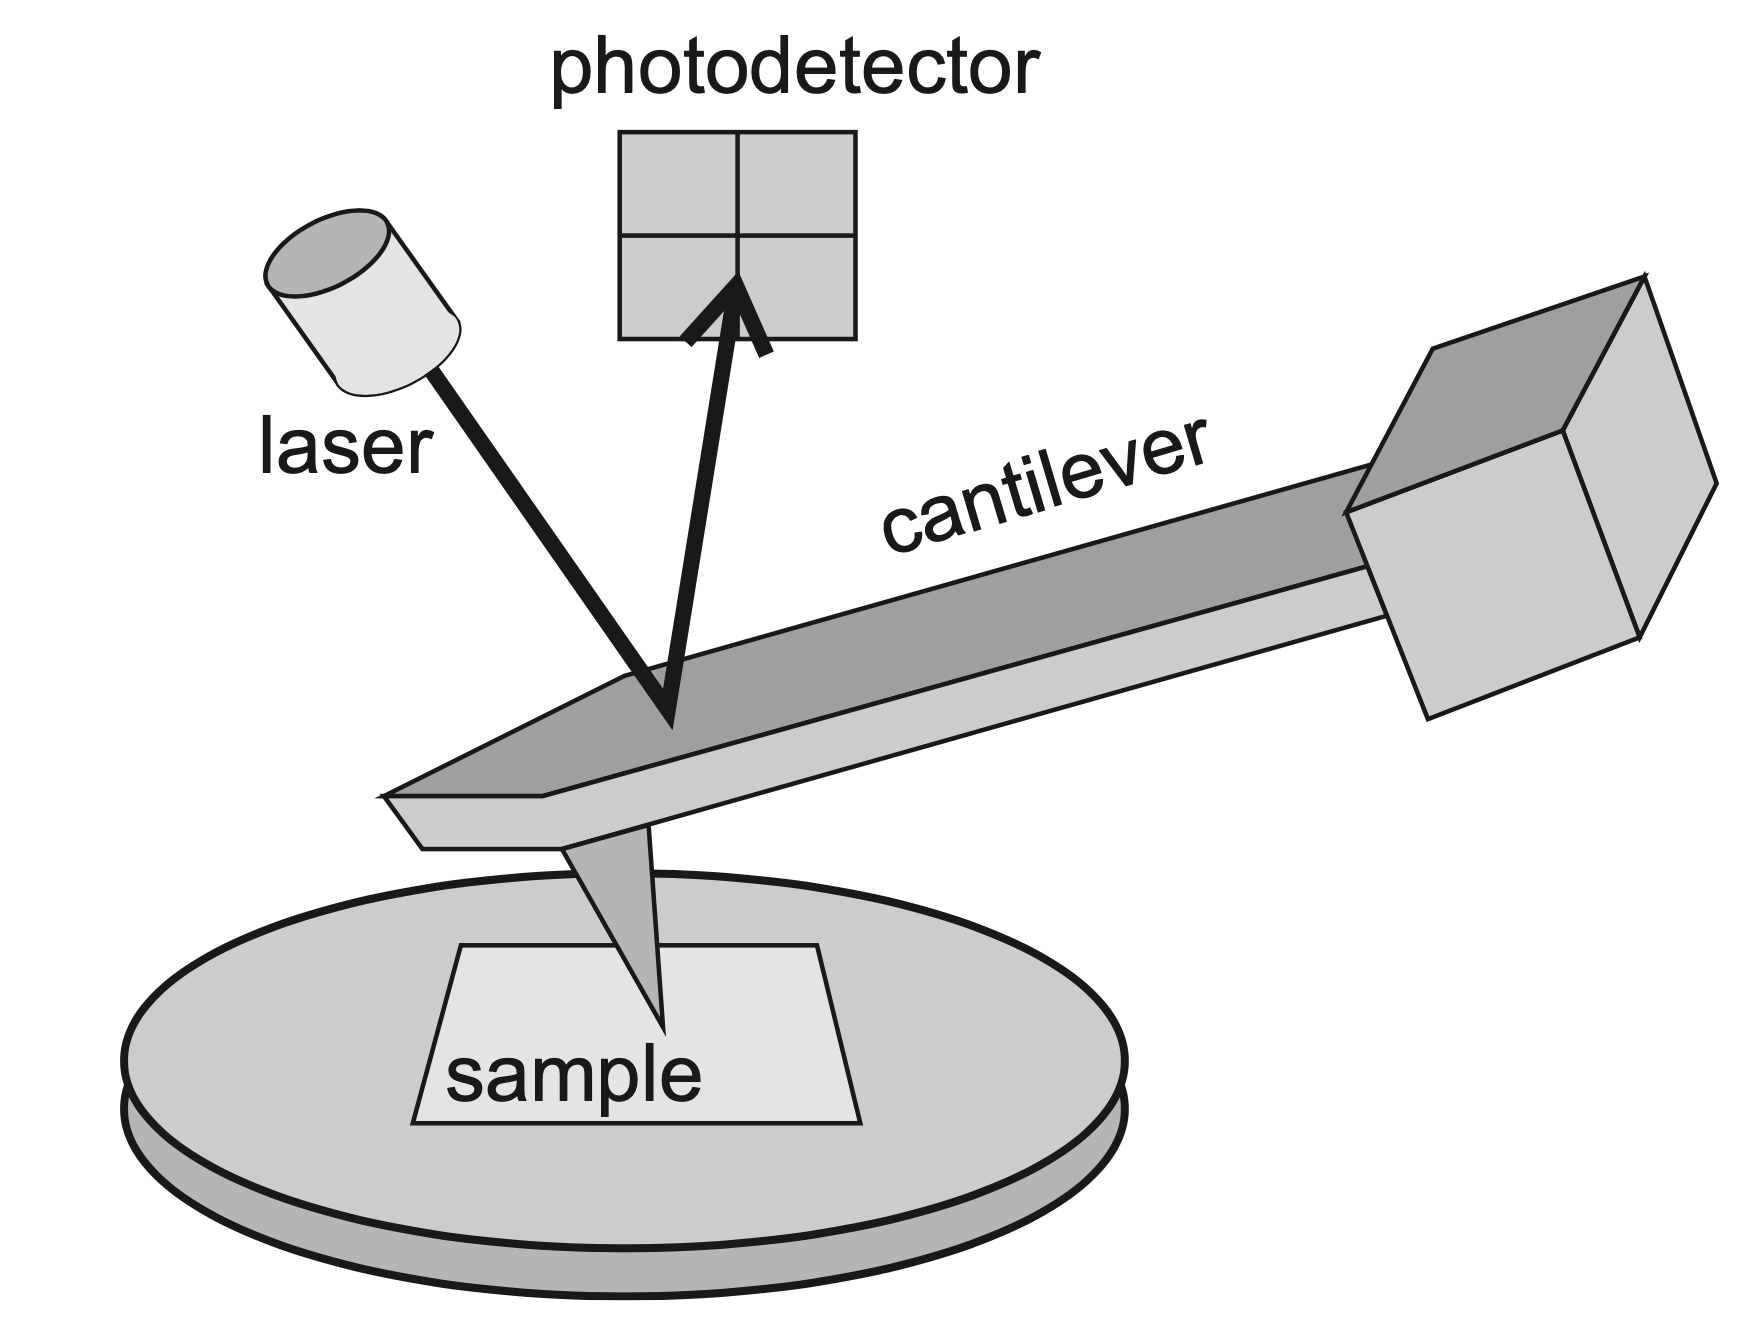
\includegraphics[width=0.6\linewidth]{figures/theory/AFM.png}
  \caption{\hl{Temporary} figure from~\cite[p. 184]{gnecco_meyer_2015}}
  \label{fig:AFM}
\end{figure}


\acrshort{AFM} can also be used to drag a nanoflake across the substrate as done by
Dienwiebel et al.~\cite{DIENWIEBEL2005197}, where a graphene flake was attached
to a \acrshort{FFM} tip and dragged across graphite. Notice that this makes the normal
loading concentrated to a single point on the flake rather than achieving an evenly distributed load. 



\subsubsection{Surface Force Apparatus}
The Surface force apparatus \acrshort{SFA} is based on two curved molecularly smooth surfaces brought into contact~\cite[p. 188]{gnecco_meyer_2015}. The sample is placed in between the two surfaces as a lubricant film for which the friction properties can be studied by applying a tangential force to the surfaces. 




\section{Summary of previous results}\label{sec:prev_results}
Several studies have investigated the frictional behavior of graphene by varying
different parameters such as normal force, sliding velocity, temperature,
commensurability and graphene thickness~\cite{penkov_tribology_2014}. In
general, we find three types of relevant systems being studied: 1) An
\acrshort{FFM} type setup where the graphene, either resting on a substrate or
suspended, is probed by an \acrshort{AFM} tip scanning across the surface. 2) A
\acrshort{SFA} setup with the graphene ``sandwiched'' in between two
substrate layers moving relative to each other using the graphene as a solid
lubricant. 3) A graphene flake sliding on a substrate, either being dragged by
an \acrshort{AFM} tip or by more complex arrangements in numerical simulations.
Considering that even the sharpest \acrshort{AFM} tip will effectively put
multiple atoms in contact with the sample, all methods are relatable to the study of nanoscale surface contacts. However, the \acrshort{FFM} type is more reminiscent of asperity theory as we expect it to deform with increasing load, while the latter two are more aligned with the Prandtl–Tomlinson type models and our specific system of interest. Nonetheless, we will consider results across all three types of systems with the relevant studies summarized in \cref{tab:friction_ref} for convenience. 


\begin{table}[H]
  % \begin{center}
  \centering
  \caption{\hl{Update multirow line span after completing the table...}}
  \label{tab:friction_ref}
  \begin{tabular}{ |M{1cm}|M{1cm}|M{1.5cm}|X{2.5cm}|X{4cm}|X{4cm}| } \hline
  System & Type & Year & Researcher & Materials & Keywords \\ \hline
  \parbox[t]{2mm}{\multirow{12}{*}{\rotatebox[origin=c]{90}{FFM}}} & \multirow{3}{*}{Exp.} & 2007~\cite{zhao_thermally_2007} & Zhao et al.\ & Si\textsubscript{3}N\textsubscript{4} tip on graphite. & Temperature dependence \\ \cline{3-6} 
  & & 2015~\cite{Paolicelli_2015} & G. Paolicelli et al.\ & Si tip, graphene on SiO2 and Ni(111) substrate  & Layers, load, shear strength \\ \cline{2-6} 
  & \multirow{4}{*}{Both}& 2019~\cite{zhang_tuning_2019} & Zhang et al.\ & Monolayer graphene  & Straining sheet \\ \cline{3-6} 
  &  & 2019~\cite{Vazirisereshk_2019} & Vazirisereshk et al.\ & Graphene,  MoS\textsubscript{2} and Graphene/MoS\textsubscript{2} heterostructure & Low friction? \\ \cline{2-6} 
  & \multirow{4}{*}{Num.} & 2015~\cite{Yoon2015MolecularDS} & Yoon et al.\ & Si tip, graphene on SiO\textsubscript{2} & Stick-slip: tip size, scan angle, layer thickness, substrate flexibility \\ \cline{3-6} 
  & & 2016~\cite{li_evolving_2016} & Li et al.\ & Si tip, graphene on a-Si substrate & Increasing layers \\ \cline{1-6} 
  \parbox[t]{2mm}{\multirow{3}{*}{\rotatebox[origin=c]{90}{SFA}}} & \multirow{4}{*}{Num.} & 2011~\cite{Wijn_2011} & Wijn et al.\ & Graphene flakes between graphite  & Rotational dynamics, superlubricity, temperature  \\ \cline{3-6} 
  & & 2012~\cite{Kim_2012} & H.\ J.\ Kim and D.\ E.\ Kim. & Carbon sheet  & Corrugated nano-structured surfaces  \\ \cline{1-6} 
  \parbox[t]{2mm}{\multirow{12}{*}{\rotatebox[origin=c]{90}{Flake}}} & \multirow{3}{*}{Exp.} & 2005~\cite{DIENWIEBEL2005197} & Dienwiebel et al.\ & Graphene on graphite & Commensurability, superlubricity  \\ \cline{3-6} 
   &  & 2013~\cite{feng_superlubric_2013}  & Feng et al.\ & Graphene on graphite &  Free sliding  \\ \cline{2-6} 
   & \multirow{9}{*}{Num.} & 2009~\cite{bonelli_atomistic_2009} & Bonelli et al.\ & Graphene on graphite  & Tight-binding, commensurability, load, flake size \\ \cline{3-6} 
   &  & 2012~\cite{Reguzzoni_2012} & Reguzzoni et al.\ & Graphene on graphite & Graphite thickness  \\ \cline{3-6} 
   &  & 2014~\cite{liu_high-speed_2014} & Liu et al.\ & Graphene on graphite & Thickness, deformations, high speed \\ \cline{3-6} 
   &  & 2018~\cite{zhu_study_2018} & P. Zhu and Li & Graphene on gold & Flake size, commensurability  \\ \cline{3-6} 
   &  & 2019~\cite{ma12091425} & Zhang et al.\  & Graphene on diamond & Temperature, sliding angle, friction coefficient  \\ \cline{1-6} 
  \end{tabular}
  % \end{center}
\end{table}


% Stick-slip
One of the earliest tribological simulations of graphene was carried out by
Bonelli et al.~\cite{bonelli_atomistic_2009} in 2009 using a tight-binding
method (excluding thermal excitations) to simulate a graphene flake on an
infinite graphene sheet~\cite{penkov_tribology_2014}. They implemented a
\acrshort{FKT}-like setup where each atom in the flake is coupled horizontally
to a rigid support by elastic springs. They recovered the stick-slip behavior,
which is also observed in \acrshort{FFM} setups both experimentally
\cite{zhao_thermally_2007, zhang_tuning_2019} and numerically
\cite{li_evolving_2016, zhu_study_2018}. Moreover, they found an agreement with
the qualitative observation that soft springs allow for a clean stick-slip
motion while hard springs ($\sim \SI{40}{N/m}$) inhibited it, which also aligns
with the Prandtl–Tomlinson model. In \acrshort{AFM} and \acrshort{SFA} experiments,
the stick-slip motion tends to transition into smooth sliding when the speed
exceeds $\sim \SI{1}{\mu/s}$ while in \acrshort{MD} modeling the same transition
is observed in the $\sim \SI{1}{m/s}$ region~\cite{Manini_2016}. More precisely
Liu et al.~\cite{liu_high-speed_2014} findes the transistion \acrshort{MD}
simulations at \SI{15}{m/S}. This 6-order-of-magnitude discrepancy has been
largely discussed in connection to simplifying assumptions in \acrshort{MD}
simulations. On the other hand, the Prandtl–Tomlinson model qualitatively disagrees
as it predicts smooth sliding for low speeds and stick-slip for high speeds.
However, in an extension of the Prandtl–Tomlinson for the study of nanoscale rolling
friction by Sircar and Patra~\cite{Sircar_2020}, they found smooth sliding for
high speeds.


% Commensurability
Bonelli et al.~\cite{bonelli_atomistic_2009} also found that commensurability,
through orientation of the flake and the direction of sliding, had a great
impact on the frictional behavior which generally aligns with the predictions of
the \acrshort{FK} and \acrshort{FKT} models. They confirmed qualitatively the
observation of superlubricity for certain incommensurable orientations which has
been reported in experiments by Dienwiebel et al.\cite{DIENWIEBEL2005197} and
further supported by experimental measurements of interaction energies by Feng
et al.~\cite{feng_superlubric_2013}. The importance of commensurability is also
reported for \acrshort{MD} simulations~\cite{ma12091425, zhu_study_2018,
Wijn_2011}. Bonelli et al.\ found the friction force and coefficient to be one
order of magnitude higher than that of the experimental results which they
attribute to the details of the numerical modeling. Generally, the experimental
coefficients between graphite and most materials lie in the range of 0.08--0.18
\cite{DIENWIEBEL2005197}. While Dienwiebel et al.~\cite{DIENWIEBEL2005197}
reported a wide range of frictional forces from $28 \pm 16$ pN to $453 \pm 16$
pN with loads $\sim [-10, 20] nN$, the change in friction with applied load was
as low as 0.05--0.4 \% for the incommensurable orientations. When using the slope definition for the frictional coefficient \cref{eq:mu_def2}, this corresponds to a coefficient in the range of 0.0005--0.004. Bonelli et al.\ attribute the low dependency to a lacking change in contact area as the flake is loaded. 

% Flake size
Furthermore, Bonelli et al.~\cite{bonelli_atomistic_2009} found friction to decrease with increasing flake size which is also reported in \acrshort{MD} simulations for graphene on gold~\cite{zhu_study_2018}. Bonelli et al.\ mainly attribute this to boundary effects, but also note that the coupling to the support made for decreased rotational freedom as flake size was increased. Thus, they hypothesized that the decreased freedom led to the graphene taking a more forced path which is associated with a decreased stick-slip behavior. The general observation however, disagrees with the \acrshort{FK} and \acrshort{FKT} model which predicts the reverse; an increase in friction with increasing size. 

An additional numerical study of monolayer islands of krypton on copper by
Reguzzoni and Righi~\cite{PhysRevB.85.201412}, supports the importance of
commensurability regarding size effects, as they report that the effective
commensurability increase drastically below a critical flake radius on the order
of $10$ Å. In a numerical study by Varini et al.~\cite{Varini_2015}, based on
Kr islands adsorbed on Pb(111), this is further elaborated as they found that
finite size effects are especially important for static friction due to a
pinning barrier arising from the edge, preventing otherwise superlubricity due
to incommensurability. They reported a relationship $F_s \sim A^{\gamma_s}$ not
only sublinear, $\gamma_s < 1$, but also sublinear with respect to the island
perimeter, $P \propto A^{1/2}$, by having $\gamma_s = 0.25$ for a hexagonal edge
and $\gamma_s = 0.37$ when circular, indicating that only a subset of the edge
is responsible for the pinning effect. This aligns with the general change in
friction found by~\cite{zhu_study_2018} for different flake geometries (square,
triangle, circle). Additionally, Varini et al.\ found the edge pinning effect to
decrease with increasing temperature as the edge energy barriers are reduced.
Bringing all this together, the main picture forming is that flake size, which
can be related to contact area, is affecting friction through a commensurability
mechanism. If the flake is constrained in some way we might not observe the same
dependency. While flake size nor contact area is easily measured in experimental
\acrshort{FFM}, Mo et al.~\cite{mo_friction_2009} found in an \acrshort{MD} simulation that friction is proportional to contact area for an indenting sphere on a nanoscale.



% Evolution effects and graphene layers
Evolution effects, or so-called friction strengthening, are also observed. That
is, friction increases during the initial stick-slip cycles, which is observed
experimentally by Zhang et al.~\cite{zhang_tuning_2019} and numerically by Li
et al.~\cite{li_evolving_2016}. However, this is only found when having the
graphene sheet resting on a substrate~\cite{zhang_tuning_2019}, as opposed to a
suspended sheet. It is also found to diminish with an increasing number of
graphene layers stacked (graphite)~\cite{li_evolving_2016}. In the study by Li
et al., they reported a general decrease in friction with an increasing number of layers which is found in other \acrshort{MD} studies~\cite{Yoon2015MolecularDS} and experimental studies as well~\cite{Filleter_2009, Lee_2010}. However, we also found an \acrshort{MD} study reporting the opposite trend~\cite{Reguzzoni_2012}.


% Accurate FFM measurements on few-layer graphene systems show that friction
% decreases by increasing graphene thickness from a single layer up to 4-5 layers,
% and then it approaches graphite values [97, 99, 101, 107, 108]. (Current trends
% in the physics of nanoscale friction)



% Deformations
A few numerical studies investigate friction under mechanical deformations. 
Zhang et al.~\cite{zhang_tuning_2019} found that straining a suspended graphene sheet will lower the kinetic friction. They attribute this to modulation of flexibility which consequently changes the local pinning capability of the contact interface. Liu et al.~\cite{liu_high-speed_2014} carried out an \acrshort{MD} simulation of high-speed ($\SI{400}{m/s}$) ballistic nanofriction of graphene on graphite. They found that a biaxial stretching of the graphitic substrate could be used to suppress frictional scattering and achieve persistent superlubricity. Another surface manipulating study was performed by H.\ J.\ Kim and D.\ E.\ Kim~\cite{Kim_2012} who investigated the effects of corrugated
nano-structured surfaces. The study revealed that corrugated surfaces with altered contact areas and structural stiffness could result in both increased or slightly decreased friction under certain load ranges. Altogether these studies highlight the importance of surface structure and mechanical conditions. 


% Normal load
The friction dependency of normal load turns out to be a complex matter and has
proven to be a highly system-dependent feature. As already mentioned, asperity
theory mainly points to a sublinear relationship between friction and load,
while the reduced-models point to a more intricate relationship through
the change of the effective substrate potential which leads to an altering of
the commensurability and the phonon dynamics. Experimentally rather different trends have been observed, although the majority agree on increasing friction with
increasing load~\cite[p. 200]{gnecco_meyer_2015}. For the graphene flake,
Dienwiebel et al.~\cite{DIENWIEBEL2005197} found a seemingly non-dependent
relationship while \acrshort{FFM} study by G. Paolicelli et al.\
\cite{Paolicelli_2015} found a sublinear relationship matching the predictions of
Maugis-Dugdale theory $(F_f \propto (F_N - F_{N,0})^{2/3})$. The discrepancy
might be attributed to the difference in system type; A spherical tip indenting the graphene sheet as opposed to the atomic flatness of the graphene-graphite
interface, which does not make for a changing contact area under load. However,
numerical studies using a graphene-graphite interface still find both sublinear
\cite{bonelli_atomistic_2009} and linear~\cite{ma12091425, zhang_tuning_2019}
load dependencies. 

In an experimental \acrshort{FFM} study by Deng et al.\ it was discovered that
the friction force kept increasing after unloading the probe tip from the
graphite surface. This has been argued to be a more general phenomenon
related to hysteresis in the adhesive interaction between two sliding bodies
\cite{thormann_negative_2013}. Following the slope definition for the friction
coefficient, these results correspond to a negative friction coefficient. More recently, a negative friction coefficient has also been observed for the loading phase by Liu et al.~\cite{Liu_2020} in an experimental study of the interface between graphite and muscovite mica heterojunction. With supporting numerical modeling this is attributed to ``synergetic and nontrivial redistribution of water molecules at the interface''. Similar results are also reported numerically by~\cite{Mandelli_2019} for graphite in contact with hexagonal boron nitride heterojunctions which is attributed to ``load-induced suppression of the moiré superstructure out-of-plane distortions leading to a less dissipative interfacial dynamics''. Thus, the concept of a negative friction coefficient has been proven for the unloading phase of adhesive contacts and in the loading phase for a few systems. 

% Speed
The dependency of velocity is generally found to increase logarithmically with
velocity in experimental \acrshort{AFM} studies~\cite[p. 201]{gnecco_meyer_2015}
which match the low-velocity regime of the Prandtl–Tomlinson type models. At higher
velocities, thermally activated processes are less important and friction becomes
independent of velocity according to the Prandtl–Tomlinson model result \cref{eq:F_thermal_ac} when ignoring the athermal regime. Saturation of the velocity dependency has been observed numerically for Si tips interacting with diamond, graphite and amorphous carbon surfaces respectively with scan velocities above \SI{1}{\mu/s}~\cite{zworner1998velocity}.  Guerra et al.~\cite{Guerra_2010}, studying gold clusters on graphite using \acrshort{MD} simulations, found a viscous friction response, friction being proportional to sliding velocity, in both low and high speed domains. However, thermal effects reversed as they found friction to decrease with increasing temperature at low speed (diffusive regime), but for high speed (ballistic regime) they found an increasing friction with temperatur. In the \acrshort{MD} simulations this crossover from ballistic to diffusive occurred between 10 and \SI{1}{m/s}. 


% Temperature
Regarding temperature itself, the general experimental trend is decreasing friction with increasing temperature as found by Zhao et al.~\cite{zhao_thermally_2007} in a series of \acrshort{AFM} graphene on graphite experiments yielding $F_{\text{fric}} \propto \exp{(1/T)}$. This agrees with the thermal drift regime of the Prandtl–Tomlinson model even though the exact temperature range does not agree. Morevoer, Wijn et al.~\cite{Wijn_2011} found that friction commensurability can be lost at higher temperatures (above 200K) where they found a power law behavior $F_k \propto T^{-1.13 \pm0.04}$. Numerically, Zhang et al.~\cite{ma12091425} found that friction increased with temperature, using a sliding speed of \SI{10}{m/s}. Considering the findings of~\cite{Guerra_2010} this qualitative different behavior might be attributed to an \acrshort{MD} related effect associated with the transition from low speed diffusive behavior as to high speed ballistic behavior.
\\
\\
From the review of previous results, we find several gaps and discrepancies in
the description of friction provided by the reduced-models, \acrshort{MD}
simulations and experimental methods respectively. Some of the discrepancies can
be attributed to the fact that different physical mechanisms are included in the
numerical modeling. The reduced-models provides the simplest description while
\acrshort{MD} simulations are thought to capture a more complex behavior. On the
other hand, we might also point differences in the studied systems as an
important factor to consider. This regard the physical conditions such as
sliding speed and temperature, but also higher level features converning the
mechanical properties of the system. For instance, the \acrshort{FFM} based
results consider an asperity-like system where the tip is expected to deform
under loading, which gives rise to a change in contact area. This feature is
lacking in the flat flake-/sheet-systems, and thus we might question the role of
the contact area in these systems. More precisely, when inflicting an
out-of-plane buckling through Kirigami cuts and stretching, the contact area is
expected to decrease as well. From asperity theory we might simply hypothesize
that friction will decrease during such a transition. However, as the system
deforms we can also expect a modification of the commensurability, and the local loading which can be associated with radical changes in the frictional behavior associated with different stick-slip regimes. From the results of a non-Kirigami sheet under tension, we already see clues that the stretching will provide an reduction in friction without considering the contact area. Similar, the results from a corrugated nano surface also points to the fact that surface stiffness might play an important role as well. 








% The theoretical framework outlined above has ex- plained a number of FFM experimental results on single crystal surfaces (Gnecco et al., 2000; Riedo et al., 2003; Stills and Overney, 2003). Furthermore, the statistical distribution of friction forces was measured to match pre- dictions from the PT model (Schirmeisen et al., 2005). These results provide strong evidence that atomic stick- slip in FFM is attributable to thermally activated slip out of a local minimum as described by the PT model. Thermally activated stick-slip friction is only seen in MD at sufficiently low speeds, which are so far only achievable through accelerated MD (Li et al., 2011a). At higher speeds, friction is mostly determined by dissipative ather- mal dynamical processes, which correspond to a funda- mentally different regime of sliding. This limits severely the regime of validity of comparisons of the PT model with MD simulations.
% https://arxiv.org/abs/1112.3234v4



%  being considered. For instance, the asperity models assume as deformation that changes contact area under loading while such an mechanism is missing for the atomic flat contact. However, this leaves a question of whether a introduced reduction of the contact area will result in a decrease in friction. Considering that both an increasing and decreasing friction are associated to the flake size of an atomic smooth contact surface, it is not obvios how this change in contact area will behave. Furthermore, the commensurability seems to be a common denominator for many explanations 


% How can we get a stable system.

% , this remain an relevant topic.



% \hl{På slutten av 2.5 trenger du et avsnitt som oppsummerer litt hva som er relevat for din studie, og som skaper en myk overgang til ``Research questions''. Men 2.5 skaper et veldig godt grunnlag for å lage research questions, siden det er mange forskjellige resultater, og du dermed kan gripe tak i motsetninger mellom tidligere eksperimenter, som dine simuleringer kan gi nye innsikter til. Jeg ville prioritert en del tid på å få til en god avslutning på 2.5 og en fin overgang til 2.6.}


% Non rigid flake which could deform and rotate,
% but(?) the graphene flake was fixed at a certain angle after applying normal
% force to reproduce \acrshort{AFM} experiments. They found stick-slip behvaiour.
% The flake size and ``stacking angle'' affected the frictional behavior, such
% that a large area resulted in experienced less friciton due the idea that the
% reactive atoms at the boundary were dominant in increasing friction. The
% influence of the stacking angle was attributed to the commensurability effect
% highlighted by the \acrshort{FK} model. Similar bahviour in various structures
% such as carbon nano tubes CNT and mica (what is mica) have previously been
% reported~\cite[41-42]{penkov_tribology_2014}. It has also been found that
% graphene (the ideal nano-structure) exhibits superlubricity in cases of lattice
% mismatch.

% % Thickness of graphene substrate
% Reguzzoni et al.~\cite[33]{penkov_tribology_2014} carried out a MD simulation of a graphene flake sliding sliding over a multi-layer (1-4) graphite substrate. They found that out-of-plane deformation of the graphene sheet (which one) increased with an increasing number of graphene layers. Meaning, that the vertical contatc stifness decreased with graphene thickness. Because frictional force and stick-slip motion were found to increase with decreasing stifness if was concluded that the single layer graphene were the best candidate for a solid nano-lubricant film. Moreover, the authors reported that the out-of-plane deformation nd the shear deformation induced by the stick-slip motion were the dominant factors incluencing friction.  


% %CNT probing suspended graphene sheet
% Smolyanitsky et al.~\cite[34]{penkov_tribology_2014} performed a \acrshort{MD} simulation of a CNT probing a suspended graphene sheet. They found that for a positive normal force the friction generally increased with normal force, while for a negative normal force (as the tip pulled the suspended graphene due to adhesion) the friction increased for a decreasing normal force. This is in practive signs of a negative friction coefficient the negative range of normal load.  


% Various simulation methods such as Molecular Dynamics (MD), Monte Carlo and ab initio calculations have been applied to investigate the diverse characteristics of graphene~\cite{penkov_tribology_2014}. Especially \acrshort{MD} simulations for tribological properties have been used in the recent years.


% --- Lowering friction with strain --- %
% Tuning friction to a superlubric state via in-plane straining


% Also~\cite{gao_frictional_2004} might be useful to go through again

% Maybe rememeber to talk about the properties of asperity systems as the sheet creates asperities as it buckles. 

% Include "Molecular dynamics simulation of atomic-scale frictional behavior of corrugated nano-structured surfaces" somewhere.

% The structural setup of our simulation is most reminiscent a graphene flake sliding on a substrate. This has been studied numerically in molecular dynamic simulations by Zhu and Li~\cite[2018]{zhu_study_2018} for a graphene flake on a gold substrate and by Zhang et al.~\cite{ma12091425}(2019) on a diamond substrate, and in a tight-binding simulation by Bonelli et al.~\cite{bonelli_atomistic_2009}(2009) for graphene on graphite. Experimental studies of a graphene flake attatched to an AFM is done by Dienwiebel et al.~\cite[2005]{DIENWIEBEL2005197} and Feng et al.~\cite[2013]{feng_superlubric_2013} sliding on graphite, but these are mainly concerned with superlubricity due to flake oreientation commensurability. 

% In our study we simmulate a graphene flake on a silicon substrate which deviates slightly from the above-mentioned references by having a different material combination. Additionally, the normal force is only applied to the ends of the sheet which might have an important effect. Obviously stretching and cutting the sheet will seperate our study dramatically from the references, but we aim to compare the frictional properties to the references before applying stretch or cuts. 



% ---- Quantitative --- %

% See comparison on friction coef in the one with diamond study 





% By consulting with the most related numerical and experimental studies, while also considering the theoretical gap between smooth atomic contact and asperity theory, we have summarized an evaluation of the most important quantative trends expected from our numerical results in \cref{var_dep}. 







% Look for source on affect on friction when stretching. Since we control the area through that there might be a stretch effect that is even stronger. 





% 

% Hint for explaining increase with stretch: Both micro-tribotester and AFM were used to investigate the micro/nano frictional behavior. It was reported that contact angle between the groove and the pin affected the frictional characteristics significantly. High contact angle led to a sudden increase in the frictional force due to interlocking mechanism.~\cite{kim_nano-scale_2009}
% These works suggest that frictional behavior at micro/nano scale is very much dependent on the surface structure and topography. Furthermore, the contact geometry between the tip and the surface such as area and orientation of the contacting angle affect the frictional force significantly.~\cite{kim_nano-scale_2009}



% Should period macth the lattice spacing as described in~\cite{kim_nano-scale_2009}[p. 144]



% Maybe talk about the slip line as shown in \cref{fig:slip_line}


% \begin{figure}[H]
%   \centering
%   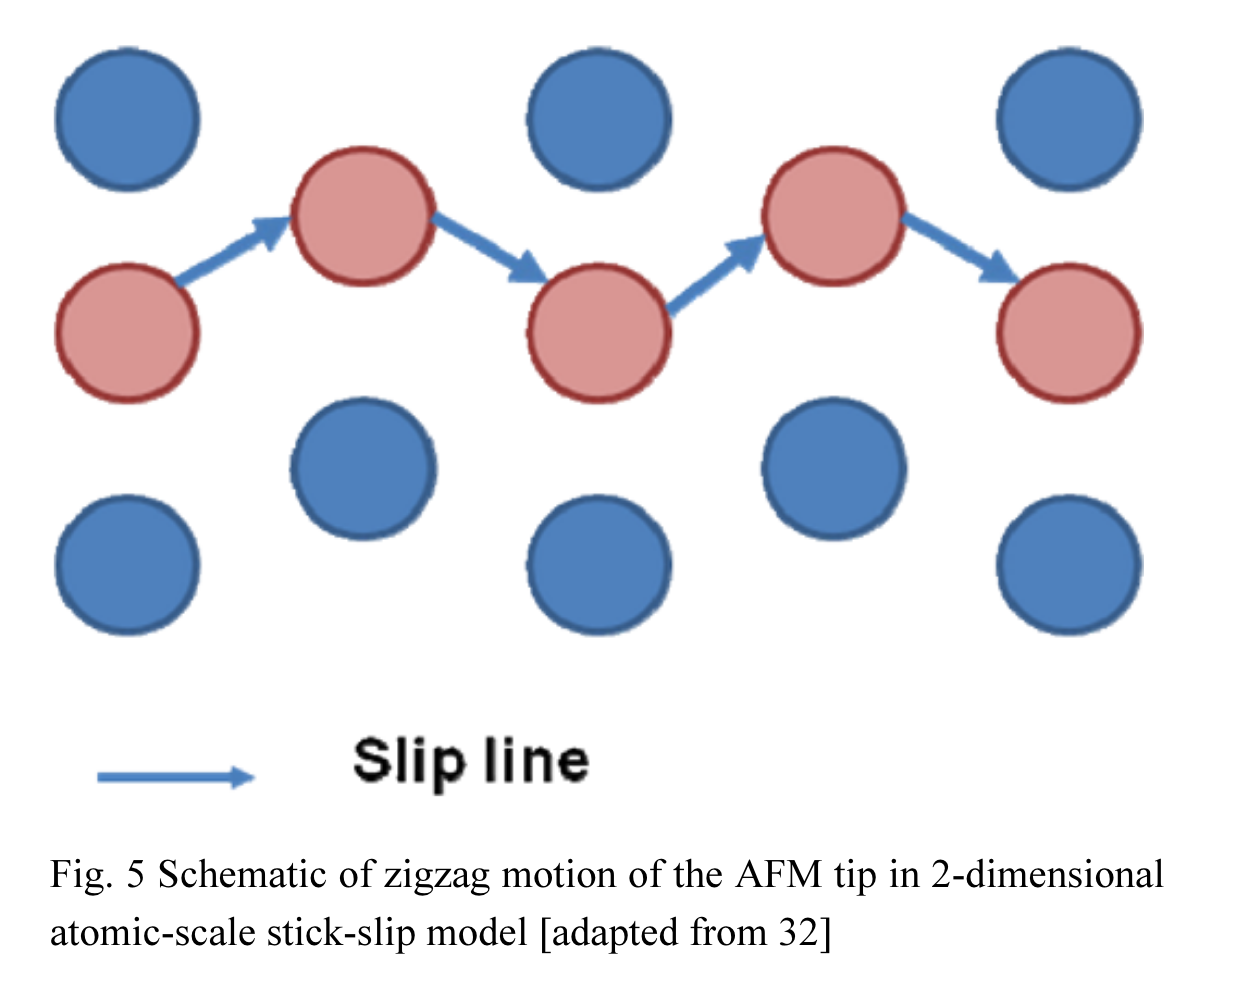
\includegraphics[width=0.5\linewidth]{figures/theory/slip_line.png}
%   \caption{\hl{Temporary} figure from~\cite{kim_nano-scale_2009}[p. 144]}
%   \label{fig:slip_line}
% \end{figure}


% the smallest force needed to set a slider in motion – is also dependent on the simulation time (a longer wait may lead to depinning when a short wait might not), and generally dependent on system size, often increasing with sub-linear scaling with the slider’s contact area. To address this kind of behavior in MD simulations, it is often necessary to resort to scaling arguments in order to extrapolate the large-area static friction from small-size MD simulations [131, 140]~\cite{Manini_2016}.


% Section 15.3. As shown in Section 15.1, the maximum value of the static friction and the slope of the turning points of the F(x) curves can be used to determine the corrugation U0 of the tip–surface interaction potential and the effective lat- eral stiffness k of the system. From Fig. 18.1(b) we estimate U0 ≈ 0.22 eV and k ≈1N/m.~\cite{gnecco_meyer_2015} p. 197






% Concerning stick-slip friction, another problem is that, unlike simulations, real experiments contain mesoscale or macroscale component intrinsically involved in the mechanical instabilities of which stick-slip consists. Here the comforting observation is that stick-slip is nearly independent of speed, so that so long as a simulation is long enough to realize a sufficient number of slip events, the results may already be good enough [148] ~\cite{Manini_2016}.


% A serious aspect of stick-slip friction which MD simulation is unable to attack is ageing. The slip is a fast event, well described by MD, but sticking is a long waiting time, during which the frictional contact settles very slowly. The longer the sticking time, the larger the static friction force necessary to cause the slip. Typicall experiments show a logarithmic increase of static friction with time [150]~\cite{Manini_2016}.

% Rate and state friction approaches, widely used in geophysics [151], describe phenomenologically frictional ageing, but a quantitative microscopic description is still lacking. Mechanisms invoked to account for contact ageing include chemical strengthening at the interface in nanoscale systems [152], and plastic creep phenomena in macroscopic systems [153].~\cite{Manini_2016}.


% See ``Selected Results of MD Simulations'' in~\cite{Manini_2016} p. 24.

% \section{Real life experimental procedures}
% From Introduction to Tribology, Second Edition, p. 526: \par The surface force
% apparatus (SFA), the scanning tunneling microscopes (STM), and atomic force and
% friction force microscopes (AFM and FFM) are widely used in nanotribological and
% nanomechanics studies.



\section{Research questions}\label{sec:research_questions}
Based on the review of friction presented in \cref{chap:friction}, it is evident that the behavior of friction is significantly influenced by various factors, such as the specific system under investigation, the numerical modeling approach, and the physical conditions related to the environment and the probing of friction. In our study, we aim to investigate the frictional behavior
of a Kirigami sheet under the effects of strain. Previous studies have
demonstrated that strained Kirigami sheets are prone to exhibiting out-of-plane buckling~\cite{PhysRevLett.121.255304, PhysRevResearch.2.042006} which is indicative of a possible transition between two distinct systems: an atomically flat interface and an asperity system. These systems are usually only studied
separately, and thus our primary objective is to explore the potential frictional effects associated with system transitions resulting from the straining of a Kirigami sheet. In particular, we want to investigate the significance of the contact area and evaluate the hypothesis that reducing the contact area will lead to a decrease in friction. Additionally, we seek to examine the relationship between the friction-load curve and this phenomenon. For the sake of contributing new insight to the field of nanoscale
friction, we are especially interested in non-linear dependencies between
friction and stretching of various Kirigami designs. Drawing on this
perspective, we aim to investigate the prospects of achieving a negative friction coefficient for a system of coupled load and stretch. The relevant
understanding of how physical conditions affect frictional behavior in
experimental and numerical studies will be considered in order to frame our
results within the theoretical understanding.

To gain a more comprehensive understanding of the potential applications of Kirigami design, we aim to develop a dataset based on \acrshort{MD} simulations that capture the frictional effects on Kirigami designs when subjected to stretching and loading. We intend to employ machine learning techniques to discern any meaningful trends in the data that may be used to inform future research endeavors. Specifically, we seek to leverage the machine learning model to facilitate an accelerated search for optimizing specific frictional properties. Our focus will be on evaluating the prospects of reducing or increasing the friction force, as well as reducing or increasing the friction coefficient for a coupled system of load and stretch. Our main research questions can be summarized as follows.


\begin{enumerate}
  \item  How can we design an \acrshort{MD} simulation that provides a reliable foundation for an investigation of the friction behavior for a Kirigami graphene sheet sliding on a substrate? How do physical conditions such as temperature and sliding speed control the frictional behavior?
  \item How can we design an ensemble of Kirigami patterns for the investigation of its frictional properties with the scope of getting out-of-plane buckling and also randomized design features?   
  \item Can we control friction for a Kirigami sheet through pattern design and stretching of the sheet?
  \begin{enumerate}
    \item How does friction dependent on a changing contact area?
    \item How does the friction-load curve relate to stretched Kirigami sheets?
    \item Are the effects of stretching and pattern design significant when considered independently?
  \end{enumerate}
  \item Is it possible to utilize machine learning techniques to identify general trends in friction associated with Kirigami designs, stretch and load?
  \item Can we use a trained machine learning model to predict new designs through accelerated search?
  \item What are the prospects of achieving a negative friction coefficient for a system of coupled load and stretch through Kirigami design?
\end{enumerate}


% \item MD without cuts to be stable (what about physical conditions)
% \item How can we design different patterns
% \item Can we observe effects from Kirigami designs
% \item Can we observe effects from stretched Kirigami designs
% \item Can we make a ML model predict the MD simulations
% \item Can we use the model to perform an accelerated search
% \item Can we use a coupled load and stretch system to demonstrate a negative friction coefficient using our Kirigami design


% This transition can be hypothesized
% to introduce the contact area as an important factor for friction, along with
% more complex effects associated with commensurability and the mechanical
% deformations in general.



% \begin{enumerate} % Try reducing the number of points here
%   \item Define a sheet indexing that allows for a unique mapping of patterns between a hexagonal graphene lattice representation to a matrix representation suited for numerical analysis. 
%   \item  Design a \acrshort{MD} simulation procedure to evaluate the frictional properties of a given graphene sheet under specified physical conditions such as load, stretch, temperature etc. 
%   \item Find and implement suitable kirigami patterns which exhibit out-of-plane buckling under tensile load. This includes the creation of a framework for creating variations within each pattern class. Additionally, create a procedure for generating different styles of random walk patterns.
%   \item Perform a pilot study of a representative subset of patterns in order to determine appropriate simulation parameters to use for further study along with an analysis of the frictional properties shown in the subset.
%   \item Create a dataset consisting of the chosen kirigami variations and random walk patterns and analyze data trends.
%   \item Train a neural network to map from the design space to physical properties such as mean friction, maximum friction, contact area etc.\ and evaluate the performance.
%   \item Perform an accelerated search optimizing for interesting frictional properties using the \acrshort{ML} model. This should be done both through the pattern generation procedures and by following a genetic algorithm approach. 
%   \item Use the most promising candidates from the accelerated search to investigate the prospects of creating a nanomachine setup that exhibits a negative friction coefficient. 
%   \item Study certain designs of interest with the scope of revealing underlying mechanisms. This includes simple correlation analysis but also a visualization of feature and gradient maps of the \acrshort{ML} network.
% \end{enumerate}






% What kind of friction effects can be associated to the stretching of Kirigami sheets.
% \item 


% How does the contact area relate to friction as the sheet buckles during stretching. 
% \item How does stretching effect friction.
% \item How does a non-stretched kirigami effect friction.
% \item what mechanism can we recognize from our expectations. 

% In general we will aim to design a friction simulation that gives stable result. We will consider the dependencies to temperautre, speed, spring constant as a means to comparing our results with the ...


% We are going to study the behvaiour of a kirigami sheet deforming under stretching which constitute a transition between system types. We will focus on how this transition effects the frictional behaviour and how this relates to parameters such as load and contact area. From the previous results we find the main expectations to our system which in \cref{tab:exp_summary}. By considering our system behaviour against these general expectations we can bring insight into some of the discrepancies related to different theoretical predictions and aim to pinpoint where our system belongs

% Experimental method lacks from not seeing the surface contact and retrieivng accurate data for what goes ons


% Size effects, edge effects and shape effects on commensurability is worth mentioning.  

%  By applying stretching to a Kirigami sheet we might
% transition the system from an atomically flat sheet towards an asperity system.
% If we were to follow asperity theory this should result in a reduced friction.
% If not, this might provide insight into the general importance of the contact
% area.

% In addition, the deformation of the sheet will most likely be connected to
% effect the commensurability which generally found to be of great importance.
% This could probably give rise to both an increase or a decrease in friction depending on whether we transition from an incommensurable to a commensurable state or vice versa. For a Kirigami modified system the dependence on load will bring insight to the discussion of how friction depends on load with two governing
% explanations being either true contact area or commensurability. 


% The dependencies for velocity, temperature and spring constant provide a reference point for the possible friction regimes, such as stick-slip versus smooth sliding or ballistic versus diffusive motion, which is essential for a more through comparison and understanding of our results. 



% Textwidth = 484,20988 pt*0,035146 pt/cm = 17,02 % \the\textwidth
% \begin{table}[H]
%   \begin{center}
%   \caption{Summary}
%   \label{tab:exp_summary}
%   \begin{tabular}{  M{5cm}  X{12cm} } \hline
%   \textbf{Stick slip} & Generally we expect to observe periodic stick-slip motion with a period matching the lattice constant(s) involved~\cite{mo_friction_2009}. This is however expected to be inhibited by high spring stiffness for the moving support, high temperature, system size and at large velocities. For the latter, we mainly refer to a ``smooth-looking'' force trace, which can still involve slips \hl{hmmm...} \\ \\
%   % At large velocities the reduced-models suggest a multiple slip behavior while experimental results suggest smooth sliding. This discrepancy might be explained by a different definition of smooth sliding as the multiple slip regime can produce seemingly ``smooth-looking'' force traces. Additionally, it is expected that the tendency of stick-slip behvaiour is reduced by increasing temperature and for incommensurability. \\ \\
%   \textbf{Static friction} & Static friction is expected to correlate with the presence of stick-slip motion. We expect it to be most pronounced for commensurable configurations with a possible disappearance for incommensurability. Moreover, static friction is expected to increase with system size, time in stationary contact and decreasing temperature. \\ \\
%   \textbf{Commensurability} & Both static and kinetic friction is expected to be highly sensitive to commensurability, through lattice spacing, the orientation of the flake relative to the substrate and the path of sliding along the substrate. By loading, rotating, cutting and stretching the sheet we might alter commensurability as well as a change of the spring constant can alter the translational freedom during sliding leading to a similar change in commensurability. \\ \\
%   \textbf{Friction evolution} \linebreak \textbf{(Friction strengthening)} & Friction evolution is found to be present in monolayer graphene resting on a substrate, and thus we expect this to be present in our simulation setup as well.  \\ \\
%   \textbf{Negative coef} & Previous result shows that a negative friction coefficient can be done, but these were related to a different system. However, alterations through stretching and corrugation have shown that it is possible to alter friction through deformations. By introducing a coupling between load and such deformations we might be able to achieve a negative coefficient.  \\ \\
%   \textbf{Normal load} & Generally an increasing friction force is expected with increasing load. Both non-dependent, sublinear and linear relationships can be expected. \\ \\
%   \textbf{Velocity} & Generally an increasing friction force is expected with increased sliding velocity. Numerical results suggest a viscous friction $F_k \propto v$ \\ \\
%   \textbf{Temperature} & From an experimental and model-based point of view friction is expected to decrease with temperature in a power law or exponential manner. However, for \acrshort{MD} simulations the transition from a diffusive to a ballistic regime at a velocity around 1--\SI{10}{m/s} is suggested to yield increasing friction with temperature.  \\ \\
%   \textbf{Contact area} & For the non-cut sheet we do not expect to see any noticeable change in contact area during loading. For a deforming sheet that successfully changes the contact area, it is theorized to alter the friction as well in a proportional manner.  \\
%   \hline
%   \end{tabular}
%   \end{center}
% \end{table}





% Formulate the research questions guiding the reading of the thesis moving on. 





